%% LyX 2.0.0 created this file.  For more info, see http://www.lyx.org/.
%% Do not edit unless you really know what you are doing.
\documentclass[12pt,english,dvips]{report}
\usepackage[T1]{fontenc}
\usepackage[latin9]{inputenc}
\setcounter{secnumdepth}{3}
\setcounter{tocdepth}{3}
\setlength{\parskip}{0.1in}
\setlength{\parindent}{0pt}

\usepackage{array}
\usepackage{verbatim}
\usepackage{textcomp}
\usepackage{amsthm}
\usepackage{amsmath}
\usepackage{amssymb}
\usepackage{graphicx}
\PassOptionsToPackage{normalem}{ulem}
\usepackage{ulem}
%\usepackage{subfig}
\usepackage{subfigure}

\makeatletter

%%%%%%%%%%%%%%%%%%%%%%%%%%%%%% LyX specific LaTeX commands.
\pdfpageheight\paperheight
\pdfpagewidth\paperwidth

%% Because html converters don't know tabularnewline
\providecommand{\tabularnewline}{\\}
%% A simple dot to overcome graphicx limitations
\newcommand{\lyxdot}{.}


%%%%%%%%%%%%%%%%%%%%%%%%%%%%%% User specified LaTeX commands.
\usepackage[ruled]{algorithm2e}
\newtheorem{clm}{Claim}
\newtheorem{mydef}{Definition}

\@ifundefined{showcaptionsetup}{}{%
 \PassOptionsToPackage{caption=false}{subfig}}

\makeatother

\usepackage{babel}
%%%%%%%%%%%%%%%%%%%%%%%%%%%%%% User specified LaTeX commands.
%
% PROJECT: <ETD> Electronic Thesis and Dissertation Initiative
%   TITLE: LaTeX report template for ETDs in LaTeX
%  AUTHOR: Neill Kipp, nkipp@vt.edu
%     URL: http://etd.vt.edu/latex/
% SAVE AS: etd.tex
% REVISED: September 6, 1997 [GMc 8/30/10]
% 

% Instructions: Remove the data from this document and replace it with your own,
% keeping the style and formatting information intact.  More instructions
% appear on the Web site listed above.



\setlength{\textwidth}{6.5in}
\setlength{\textheight}{8.5in}
\setlength{\evensidemargin}{0in}
\setlength{\oddsidemargin}{0in}
\setlength{\topmargin}{0in}




% Uncomment for double-spaced document.
% \renewcommand{\baselinestretch}{2}

% \usepackage{epsf}

\begin{document}
\thispagestyle{empty} \pagenumbering{roman} 

\begin{center}
% TITLE
{\Large On the Design of Contention Managers for Real-Time Software
Transactional Memory}
\par\end{center}{\Large \par}

\begin{center}
\vfill{}

\par\end{center}

\begin{center}
Mohammed Elshambakey
\par\end{center}

\begin{center}
\vfill{}

\par\end{center}

\begin{center}
Preliminary Examination Proposal submitted to the Faculty of the \\
 Virginia Polytechnic Institute and State University \\
 in partial fulfillment of the requirements for the degree of
\par\end{center}

\begin{center}
\vfill{}

\par\end{center}

\begin{center}
Doctor of Philosophy \\
 in \\
 Computer Engineering 
\par\end{center}

\begin{center}
\vfill{}

\par\end{center}

\begin{center}
Binoy Ravindran, Chair \\
Robert P. Broadwater \\
 Cameron D. Patterson \\
Mohamed Rizk Mohamed. Rizk\\
Anil Kumar S. Vullikanti
\par\end{center}

\begin{center}
\vfill{}

\par\end{center}

\begin{center}
April 10, 2012 \\
 Blacksburg, Virginia
\par\end{center}

\begin{center}
\vfill{}

\par\end{center}

\begin{center}
Keywords: Software Transactional Memory, Contention Manager \\
 Copyright 2012, Mohammed Elshambakey
\par\end{center}

\pagebreak{}

\thispagestyle{empty} 

\begin{center}
{\Large On the Design of Contention Managers for Real-Time Software
Transactional Memory}
\par\end{center}{\Large \par}

\begin{center}
\vfill{}

\par\end{center}

\begin{center}
Mohammed Elshambakey
\par\end{center}

\begin{center}
\vfill{}

\par\end{center}

\begin{center}
(ABSTRACT)
\par\end{center}

\begin{center}
\vfill{}

\par\end{center}

\textbf{NEEDS TO BE WRITTEN}

\vfill{}


% GRANT INFORMATION


\pagebreak{}

% Dedication and Acknowledgments are both optional
% \chapter*{Dedication}
% \chapter*{Acknowledgments}


\tableofcontents{}\pagebreak{}

\listoffigures
\pagebreak{}

\listoftables
\pagebreak{}

\pagenumbering{arabic} \pagestyle{myheadings}


\chapter{Introduction}

\markright{Mohammed Elshambakey \hfill{}Chapter 1. Introduction
\hfill{}}

Data structure implementation affects degree of exploited parallilsm
in the system \cite{shavit2011data}. As the implementation moves
from lock-based to non-blocking, more parallilism can be exploited.
Thus, more computation speed-up, but more complex design. Things become
more complicated when it comes to synchronization under real-time
multiprocessor systems. Real-time systems should meet deadline of
each task as much as possible. With shared objects, tasks have to
execute in a serial order to some degree when accessing shared objects.
The major problem arises when one of the accesses is a \textit{write}
operation. Conflict resultion techniques is used to decide how to
access these shared objects. In lock-based systems, tasks try to obtain
an object's lock before accessing it. While in lock-free techniques,
some intuition is used to allow tasks to simultaneously access the
object without violating consistency. Different synchronization techniqes
affect response time of each task. Depending on the rationale of conflict
resolution, a task might have to wait for all other interfering tasks
before it can access the required object.

\subsection{Contribution}
We consider STM for real-time multiprocessor systems under G-EDF and
G-RMA schedulers. Atomic sections can be of arbitrary size. Earliest
deadline CM (ECM) is re-presented, and another priority-based CM (RCM)
is developed. Length-based CM (LCM) is provided to reduce retry cost
of aborted transactions. LCM depends not only on priority, but also
on relative length of the interfering transaction to the remaining
length of the interfered transaction.

%%%%%%%%%%%%%%%%%
% Include an EPS figure with this command:
%   \epsffile{filename.eps}
%%%%%%%%%%%%%%%%
% Do tables like this:


\begin{table}
\caption{The Graduate School wants captions above the tables.}


\centering{}%
\begin{tabular}{ccc}
x  & 1  & 2 \tabularnewline
\hline 
1  & 1  & 2 \tabularnewline
2  & 2  & 4 \tabularnewline
\hline 
\end{tabular}
\end{table}


%%%%%%%%%%%%%%%%%%%%%%%%%%%%%%%%



\chapter{ECM and RCM}

We consider software transactional memory (STM) for concurrency control in multicore embedded real-time software. We investigate real-time contention managers (CMs) for resolving transactional conflicts, including those based on dynamic and fixed priorities, and establish upper bounds on transactional retries and task response times. We identify the conditions under which STM (with the proposed CMs) is superior to lock-free synchronization. 

\section{G-EDF/EDF CM Response Time}
\label{sec:g-edf-edf-cm}

Since only one atomic section among many that share the same object can commit at any time under STM, those atomic sections execute in sequential order.  A task $\tau_{i}$'s atomic sections are interfered by other tasks that share the same objects with $\tau_{i}$.  
The EDF CM will abort and retry an atomic section of $\tau_i$, $s_i^k(\theta)$ due to a conflicting atomic section of $\tau_j$, $s_j^l(\theta)$, if the absolute deadline of $\tau_j$ is less than or equal to the absolute deadline of $\tau_i$. 
%%BR: I reworded. Check for accuracy. 
Hereafter, we will use \emph{ECM} to refer to a multiprocessor system scheduled by G-EDF and resolves STM conflicts using the EDF CM. 


The maximum number of times a task $\tau_{j}$ interferes with $\tau_{i}$ is given in~\cite{key-2} and is illustrated in Figure~\ref{fig1}. 
Here, the deadline of an instance of $\tau_{j}$ coincides
with that of $\tau_{i}$, and $\tau_{j}^{1}$ is delayed by its maximum
jitter $J_{j}$, which causes all or part of $\tau_{j}^1$'s execution to overlap within $T_i$. From Figure~\ref{fig1}, it is seen that $\tau_{j}$'s maximum workload that interferes with $\tau_{i}$ (when there are no atomic sections) in $T_{i}$ is:
\begin{eqnarray}
W_{ij}\left(T_{i}\right) & \le & \left\lfloor\frac{T_{i}}{T_{j}}\right\rfloor c_{j}+min\left(c_{j},T_{i}-\left\lfloor\frac{T_{i}}{T_{j}}\right\rfloor T_{j}\right)\nonumber \\
 & \le & \left\lceil\frac{T_{i}}{T_{j}}\right\rceil c_{j}\label{eq11}\end{eqnarray}

For an interval $L<T_{i}$, the worst case pattern of interference is shown in Figure~\ref{fig2}. Here, $\tau_{j}^{1}$ contributes by all its $c_j$, and $d_j^{k-1}$ does not have to coincide with $L$, as $\tau_j^{k-1}$ has a higher priority than that of $\tau_{i}$. The workload of $\tau_{j}$ is:
\begin{equation}
W_{ij}\left(L\right)\le \left(\left\lceil\frac{L-c_{j}}{T_{j}}\right\rceil +1\right)c_{j}
\label{eq12}\end{equation}

Thus, the overall workload, over an interval $R$ is:
\begin{equation}
W_{ij}\left(R\right)=min\left(W_{ij}\left(R\right),W_{ij}\left(T_{i}\right)\right)\label{eq13}\end{equation}
where $W_{ij}(R)$ is calculated by~(\ref{eq12}) if $R<T_i$, otherwise, it is calculated by~(\ref{eq11}).

\begin{figure}%[htbp]
\centering
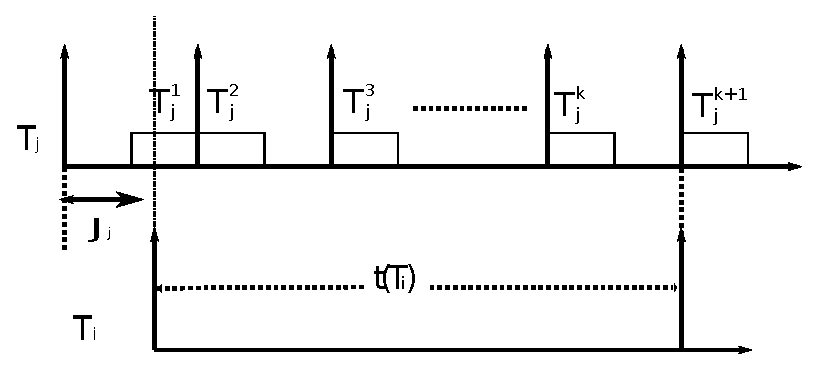
\includegraphics[bb=0bp 0bp 542bp 162bp,scale=0.5]{figures/figure9-a}
\caption{\label{fig1} Maximum interference between two tasks, running on different processors, under G-EDF}
\end{figure}


\begin{figure}
\centering
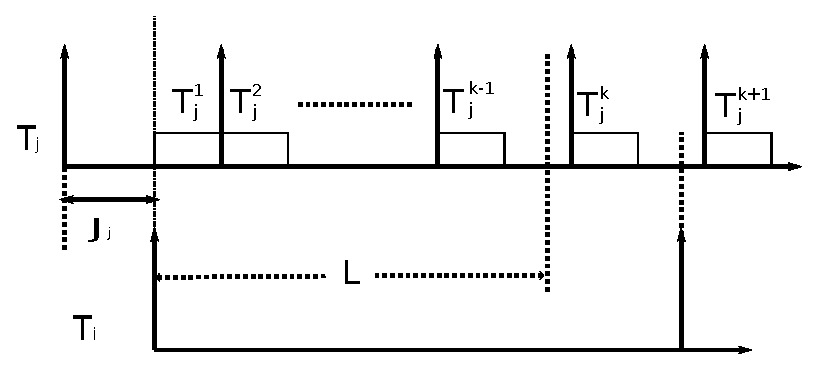
\includegraphics[bb=0bp 0bp 542bp 162bp,scale=0.5]{figures/figure9-b}
\caption{\label{fig2}Maximum interference during an interval $L$ of $T_{i}$}
\end{figure}



\subsection{Retry Cost of Atomic Sections}

\begin{figure*}
\centering
\subfigure[Early validation]{
            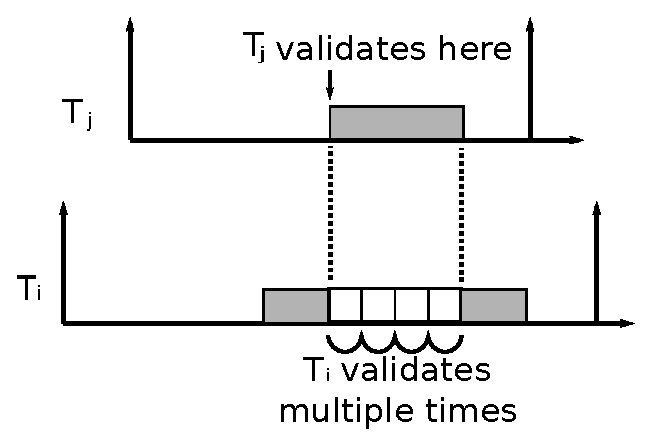
\includegraphics[scale=.45]{figures/figure5-a}
\label{fig5-a} 
}\hspace{1.2cm}
\subfigure[Lazy validation with $len(s_{i}^{k}(\theta))\le len(s_{j}^{l}(\theta))$]{
            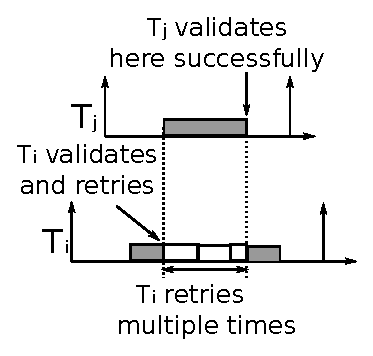
\includegraphics[scale=.65]{figures/figure5-b-1}
\label{fig5-b} 
}\hspace{1.5cm}
\subfigure[Lazy validation with $len(s_{i}^{k}(\theta))>len(s_{j}^{l}(\theta))$]{
            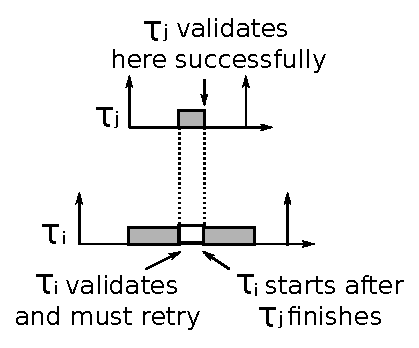
\includegraphics[scale=.65]{figures/figure5-c-1}
\label{fig5-c} 
}
\caption{Retry of $s_i^k(\theta)$ due to $s_j^l(\theta)$}  
\label{fig5}
\end{figure*}


\begin{clm}\label{gedf-edf}
Under ECM, a task $T_i$'s maximum retry cost during $T_i$ is upper bounded by:
\begin{eqnarray}
RC\left(T_{i}\right) & \le & \sum_{\theta\in\theta_{i}}\Bigg(\Big(\sum_{\tau_{j}\in\gamma_i(\theta)}\Big(\left\lceil\frac{T_{i}}{T_{j}}\right\rceil\sum_{\forall s_{j}^{l}(\theta)}len\big(s_{j}^{l}(\theta)\nonumber \\
 & + & s_{max}(\theta)\big)\Big)\Big)-s_{max}(\theta)+s_{i_{max}}(\theta)\Bigg)\label{eq3}\end{eqnarray}
\end{clm}
\begin{proof}
Consider two instances $\tau_{i}^a$ and $\tau_{j}^b$, where $d_j^b \le d_i^a$. When a shared object conflict occurs, the EDF CM will commit the atomic section of $\tau_j^b$ while aborting and retrying that of $\tau_i^a$.
Thus, an atomic section of $\tau_i^a$, $s_{i}^{k}(\theta)$,
will experience its maximum delay when it is at the end of its atomic section,  
and the conflicting atomic section of $\tau_j^b$, $s_{j}^{l}(\theta)$, starts, because the whole $s_i^k (\theta)$ will be repeated after $s_j^l (\theta)$.

Validation (i.e., conflict detection) in STM is usually done in two ways~\cite{austenmc:tcc:dissertation:2009}: a) eager (pessimistic), in which conflicts are detected at access time, and b) lazy (optimistic), in which conflicts are detected at commit time. Despite the validation time incurred (either eager or lazy),  
$s_{i}^{k}(\theta)$ will retry for the same time duration, which is $len(s_{j}^{l}(\theta)+s_i^k(\theta))$. Then, $s_i^k(\theta)$ can commit successfully  
unless it is interfered by another conflicting atomic section, as shown in Figure~\ref{fig5}. 

In Figure~\ref{fig5-a}, $s_{j}^{l}(\theta)$
validates at its beginning, due to early validation, and a conflict
is detected. So $\tau_{i}^a$ retries multiple times (because at the start of each retry, $\tau_{i}^a$ validates) 
during the execution of $s_{j}^{l}(\theta)$.
When $\tau_{j}^b$ finishes its atomic section, $\tau_{i}^a$ executes its atomic section. 

In Figure~\ref{fig5-b}, 
$\tau_{i}^a$ validates at its end (due to lazy validation), and detects a conflict with $\tau_{j}^b$.
Thus, it retries, and because its atomic section length is shorter
than that of $\tau_{j}^b$, it validates again within the execution
interval of $s_{j}^{l}(\theta)$. However, the EDF CM retries it again.
This process continues until $\tau_{j}^b$ finishes its atomic section.
If $\tau_{i}^a$'s atomic section length is longer than that of $\tau_{j}^b$,
$\tau_{i}^a$ would have incurred the same retry time, because
$\tau_{j}^b$ will validate when $\tau_{i}^a$ is retrying, and $\tau_{i}^a$ will
retry again, as shown in Figure~\ref{fig5-c}. Thus, the retry cost
of $s_{i}^{k}(\theta)$ is $len(s_{i}^{k}(\theta)+s_{j}^{l}(\theta))$.

If multiple tasks interfere with $\tau_{i}^a$ or
interfere with each other and $\tau_{i}^a$ (see the two interference examples in Figure~\ref{fig6}), then, in each case, each atomic section of the shorter deadline tasks contributes to the delay of $s_{i}^{p}(\theta)$ by its total length, plus a retry of some atomic section in the longer deadline tasks. For example,
$s_{j}^{l}(\theta)$ contributes by $len(s_{j}^{l}(\theta)+s_{i}^{p}(\theta))$
in both Figures~\ref{fig6-a} and~\ref{fig6-b}. 
%%BR: YOu should say "..in both Figures~\ref{fig6-a} and~\ref{fig6-b}." (That is, "F" must be capital case).
In Figure~\ref{fig6-b}, $s_{k}^{y}(\theta)$ causes a retry 
to $s_{j}^{l}(\theta)$, and $s_{h}^{w}(\theta)$ causes a retry to $s_{k}^{y}(\theta)$.


Since we do not know in advance which atomic section will be retried
due to another, we can safely assume that, each atomic section (that shares the same object with  $\tau_i^a$) in a shorter deadline task contributes by its total length, in addition to the maximum length between all atomic sections that share the same object, $len(s_{max}(\theta))$. Thus, 
\begin{equation}
\mbox{\ensuremath{W_{i}^{p}\left(s_{j}^{k}\left(\theta\right)\right)\le len\left(s_{j}^{k}\left(\theta\right)+s_{max}\left(\theta\right)\right)}}\label{eq2}\end{equation}


Thus, the total contribution of all atomic sections of all other tasks
that share objects with a task $\tau_i$ 
to the retry cost of $\tau_i$ during $T_i$ is:
\begin{eqnarray}
RC\left(T_{i}\right) & \le & \sum_{\theta\in\theta_{i}}\sum_{\tau_{j}\in\gamma_i(\theta)}\Big(\left\lceil\frac{T_{i}}{T_{j}}\right\rceil\sum_{\forall s_{j}^{l}(\theta)}len\big(s_{j}^{l}(\theta)\nonumber \\
 & + & s_{max}(\theta)\big)\Big)\label{eq3-1}\end{eqnarray}



Here, $\left\lceil\frac{T_{i}}{T_{j}}\right\rceil\sum_{\forall s_{j}^{l}\left(\theta\right)}len\left(s_{j}^{l}\left(\theta\right)+s_{max}\left(\theta\right)\right)$ is  the contribution of all instances of $\tau_{j}$ during $T_{i}$. This contribution is added to all tasks. The last atomic section to execute is $s_{i}^{p}(\theta)$ ($\tau_i$'s atomic section that was delayed by conflicting atomic sections of other tasks). One of the other atomic sections (e.g., $s_{m}^{n}(\theta)$) should have a contribution $len(s_{m}^{n}(\theta)+s_{i_{max}}(\theta))$, instead of $len(s_{m}^{n}(\theta)+s_{max}(\theta))$. That is why one $s_{max}(\theta)$ should be subtracted, and $s_{i_{max}}(\theta)$ should be added (i.e., $s_{i_{max}}(\theta)-s_{max}(\theta)$). Claim follows.
\end{proof}

\begin{figure*}%[htbp]%
\centering%
\subfigure[Other atomic sections interfere only with $s_i^p(\theta)$]{
            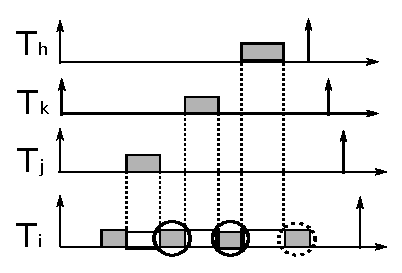
\includegraphics[scale=.65]{figures/figure6-a-1}
\label{fig6-a} 
}\hspace{1cm}
\subfigure[All atomic sections interfere with each other and $s_i^p(\theta)$]{
            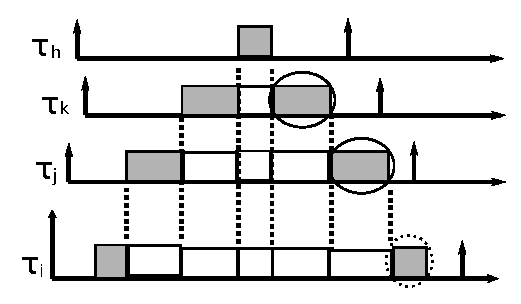
\includegraphics[scale=.6]{figures/figure6-b}
\label{fig6-b} 
}
\begin{tabular}{>{\centering}p{1cm}l}
\includegraphics[scale=0.45]{figures/circle} & Replaced in calculations by $s_{max}(\theta)$\tabularnewline
\includegraphics[scale=0.45]{figures/dotted_circle} & Replaced in calculations by $s_{i_{max}}(\theta)$\tabularnewline
\end{tabular}
\caption{Retry of $s_i^p(\theta)$ due to other atomic sections}  
\label{fig6}
\end{figure*}

\begin{clm}
Claim~\ref{gedf-edf}'s retry bound can be minimized as:
\begin{equation}
RC(T_{i})\le \sum_{\theta\in\theta_{i}}min(\Phi_1 , \Phi_2)\label{eq5}\end{equation}
where $\Phi_1$ is calculated by (\ref{eq3}) for one object $\theta$ (not the sum of objects in $\theta_i$),  and 
\begin{eqnarray}
\Phi_2 & = & \Bigg(\sum_{\tau_{j}\in\gamma_i(\theta)} \Big(\left\lceil\frac{T_{i}}{T_{j}}\right\rceil\sum_{\forall s_{j}^{l}(\theta)}len \big(s_{j}^{l}(\theta)\nonumber \\
 &  & +s_{max}^{*}(\theta) \big) \Big) \Bigg)-\bar{s}_{max}(\theta)+s_{i_{max}}(\theta)\label{eq4}\end{eqnarray}
 where $s^*_{max}$ is the maximum atomic section between all tasks, except $\tau_j$, accessing $\theta$. $\bar{s}_{max}(\theta)$ is the second maximum atomic section between all tasks accessing $\theta$.
\end{clm}
\begin{proof}
(\ref{eq3}) can be modified by noting that a task $\tau_j$'s atomic section 
may conflict with those of other tasks, but not with $\tau_j$. 
This is because, tasks are assumed to arrive sporadically, and  each instance finishes before the next begins. 
Thus, (\ref{eq2}) becomes:
\begin{equation}
W_i^p \left(s_j^k (\theta)\right)\le len\left(s_j^k (\theta)+s^*_{max}(\theta)\right)
\label{eq4-1}\end{equation}

To see why $\bar{s}{}_{max}(\theta)$ is used instead of $s_{max}(\theta)$, the maximum-length atomic section of each task that accesses $\theta$ is grouped into an array, in non-increasing order of their lengths. $s_{max}(\theta)$ will be the first element of this array, and $\bar{s}_{max}(\theta)$ will be the next element, as illustrated in Figure~\ref{fig7}, where the maximum atomic
section of each task that accesses $\theta$ is associated with
its corresponding task. According to (\ref{eq4-1}), all tasks
but $\tau_{j}$ will choose $s_{j_{max}}(\theta)$ as the value of $s_{max}^{*}(\theta)$.
But when $\tau_{j}$ is the one whose contribution is studied,
it will choose $s_{k_{max}}(\theta)$, as it is the maximum one not
associated with $\tau_{j}$. This way, it can be seen that the maximum
value always lies between the two values $s_{jmax}(\theta)$ and $s_{kmax}(\theta)$. 
Of course, these two values can be equal, or the maximum value can be associated with $\tau_i$ itself, and not with any one of the interfering tasks. In the latter case,
the chosen value will always be the one associated with $\tau_i$, which still lies between the two largest values. 

\begin{figure}[htbp]
\centering
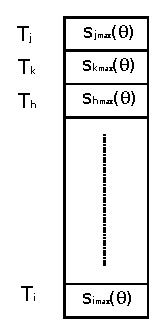
\includegraphics[scale=0.7]{figures/figure7}
\caption{\label{fig7}Values associated with $s_{max}^{*}(\theta)$}
\end{figure}


This means that the subtracted $s_{max}(\theta)$ in (\ref{eq3})
must be replaced with one of these two values ($s_{max}(\theta)$ or $\bar{s}_{max}(\theta)$). However, since we do not know  which task will interfere with $\tau_i$, the minimum is chosen, as we are determining the worst case retry cost (as this value is going to be subtracted),
and this minimum is the second maximum.

Since it is not known a-priori whether $\Phi_1$ will be smaller than $\Phi_2$ for a specific $\theta$, the minimum of $\Phi_1$ and $\Phi_2$ is taken as the worst-case contribution for $\theta$ in $RC(T_i)$. 
%Claim follows.
\end{proof}


\subsection{Upper Bound on Response Time}

To obtain an upper bound on the response time of a task $\tau_{i}$, the term $RC(T_{i})$ must be added to the workload of other tasks during the non-atomic
execution of $\tau_{i}$. But this requires modification of the WCET of each
task as follows. 
%starthere
$c_{j}$ of each interfering task $\tau_{j}$ should be inflated to accommodate the interference of each task $\tau_{k},$ $k\ne j,i$. Meanwhile, atomic regions that access shared objects between $\tau_{j}$ and $\tau_{i}$ should not be considered in the inflation cost, because they have already been calculated in $\tau_{i}$'s retry cost. Thus, $\tau_{j}$'s inflated WCET becomes:
\begin{equation}
c_{ji}=c_{j}-\left(\sum_{\theta\in(\theta_{j}\wedge\theta_{i})}len \left(s_{j}(\theta) \right) \right)+RC(T_{ji})\label{eq9}\end{equation}
where, $c_{ji}$ is the new WCET of $\tau_{j}$ relative to $\tau_{i}$; 
the sum of lengths of all atomic sections in $\tau_{j}$ that access object $\theta$ is $\sum_{\theta \in (\theta_j \wedge \theta_i)} {len(s_{j}(\theta))}$; and $RC(T_{ji})$ is the $RC(T_j)$ 
 without including the shared objects between $\tau_{i}$ and $\tau_{j}$.
The calculated WCET is relative to task $\tau_{i}$, as it changes from task to task. The upper bound on the response time of $\tau_{i}$, denoted $R_{i}^{up}$, can be calculated iteratively, using a modification of Theorem 6 in~\cite{key-2}, as follows:
\begin{equation}
R_{i}^{up}=c_{i}+RC(T_{i})+\left\lfloor\frac{1}{m}\sum_{j\ne i}W_{ij}(R_{i}^{up})\right\rfloor
\label{eq10}
\end{equation}
where $R_{i}^{up}$'s initial value is $c_{i}+RC(T_{i})$.

$W_{ij}(R_{i}^{up})$ is calculated by (\ref{eq13}), and $W_{ij}(T_{i})$
is calculated by (\ref{eq11}), with $c_{j}$ replaced by 
$c_{ji}$, and changing~(\ref{eq12}) as:
\begin{equation}
W_{ij}(L)=max\begin{cases}
\left(\left\lceil\frac{L-\left(c_{ji}+\sum_{\theta\in(\theta_{j}\wedge\theta_{i})}len(s_{j}(\theta))\right)}{T_{j}}\right\rceil+1 \right)c_{ji}\\
\left\lceil\frac{L-c_{j}}{T_{j}}\right\rceil.c_{ji}+c_{j}-\sum_{\theta\in(\theta_{j}\wedge\theta_{i})}len(s_{j}(\theta))\end{cases}\label{eq14}\end{equation}

(\ref{eq14}) compares two terms, as we have two cases:


\textit{Case 1}. $\tau_j^1$ (shown in Figure~\ref{fig2}) contributes by $c_{ji}$. Thus, other instances of $\tau_j$ will begin after this modified WCET, but the sum of the shared objects' atomic section lengths is removed from $c_{ji}$, causing other instances to start earlier. Thus, the term $\sum_{\theta\in(\theta_i\wedge\theta_j)} {len(s_{j}(\theta))}$ is added to $c_{ji}$ to obtain the correct start time. 

\textit{Case 2}. $\tau_j^1$ contributes by its $c_j$, but the sum of the shared atomic section lengths  between $\tau_i$ and $\tau_j$ should be subtracted from the contribution of $\tau_j^1$, as they are already included in the retry cost. 

It should be noted that subtraction of the sum of the shared objects' atomic section lengths is done in the first case to obtain the correct start time of other instances, while in the second case, this is done to get the correct contribution of $\tau_j^1$. The maximum is chosen from the two terms in (\ref{eq14}), because they differ in the contribution of their $\tau_j^1$s, and the number of instances after that.


\subsubsection{Tighter Upper Bound}

To tighten $\tau_{i}$'s response time upper bound, $RC(\tau_i)$ needs to be calculated recursively over duration $R_i^{up}$, 
and not directly over $T_i$, as done in (\ref{eq10}). So, (\ref{eq5}) must be changed to include the modified number of interfering instances. And if $R_i^{up}$ still extends to $T_i$, a situation like that shown in Figure
\ref{fig10} can happen.
\begin{figure}
\centering{}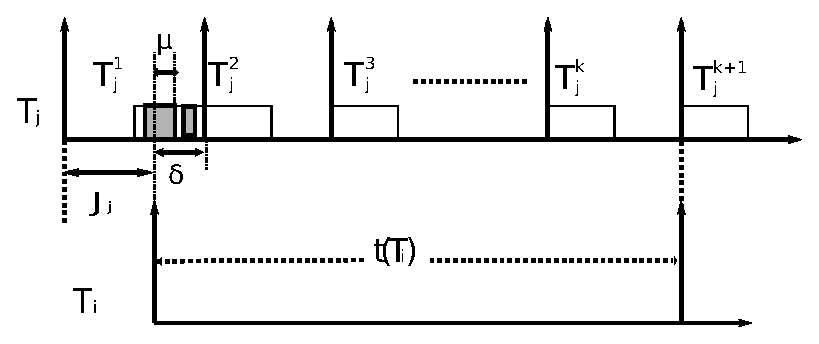
\includegraphics[scale=0.5]{figures/figure10}\caption{\label{fig10} Atomic sections of job $\tau_{j}^{1}$ contributing to period $T_i$}
\end{figure}


To counter the situation in Figure~\ref{fig10}, atomic sections of $\tau_{j}^{1}$ that are contained in the interval $\delta$
are the only ones that can contribute to $RC(T_{i})$. Of course, they can be lower, but cannot be greater, because $\tau_{j}^{1}$ has been delayed by its maximum jitter. Hence, no more atomic sections
can interfere during the duration 
$[d_j^1 -\delta,d_j^1]$.

For simplicity, we use the following notations:
\begin{itemize}
\item $\lambda_{1}\left(j,\theta\right)=\sum_{\forall s_{j}^{l}\left(\theta\right)\in\left[d_j^1-\delta,d_j^1\right]}len\left(s_{j}^{l^{*}}\left(\theta\right)+s_{max}\left(\theta\right)\right)$
\item $\chi_{1}\left(i,j,\theta\right)=\left\lfloor\frac{T_{i}}{T_{j}}\right\rfloor\sum_{\forall s_{j}^{l}\left(\theta\right)}len\left(s_{j}^{l}\left(\theta\right)+s_{max}\left(\theta\right)\right)$
\item $\lambda_{2}\left(j,\theta\right)=\sum_{\forall s_{j}^{l}\left(\theta\right)\in\left[d_{j}^{1}-\delta,d_{j}^{1}\right]}len\left(s_{j}^{l^{*}}\left(\theta\right)+s_{max}^{*}\left(\theta\right)\right)$
\item $\chi_{2}\left(i,j,\theta\right)=\left\lfloor\frac{T_{i}}{T_{j}}\right\rfloor\sum_{\forall s_{j}^{l}\left(\theta\right)}len\left(s_{j}^{l}\left(\theta\right)+s_{max}^{*}\left(\theta\right)\right)$
\end{itemize}

Here, $s_{j}^{l^{*}}\left(\theta\right)$ is the part of $s_{j}^{l}\left(\theta\right)$ that
is included in the interval $\delta$. Thus, if $s_j^l (\theta)$ is partially included in $\delta$, it contributes by its included length $\mu$.

Now, (\ref{eq5}) can be modified as:
\begin{equation}
RC\left(T_{i}\right)\le \sum_{\theta\in\theta_{i}}min\begin{cases}
\begin{cases}
\Bigl(\left(\sum_{\tau_{j}\in\gamma_i\left(\theta\right)}\lambda_{1}\left(j,\theta\right)+\chi_{1}\left(i,j,\theta\right)\right)\\
-s_{max}\left(\theta\right)+s_{i_{max}}\left(\theta\right)\Bigr)\end{cases}\\
\begin{cases}
\Bigl(\left(\sum_{\tau_{j}\in\gamma_i\left(\theta\right)}\lambda_{2}\left(j,\theta\right)+\chi_{2}\left(i,j,\theta\right)\right)\\
-\bar{s}_{max}\left(\theta\right)+s_{i_{max}}\left(\theta\right)\Bigr)\end{cases}\end{cases}\label{eq15}\end{equation}



Now, we compute $RC(L)$, where $L$ does not extend to the last instance of $\tau_{j}$. Let:
\begin{itemize}
\item $\upsilon\left(L,j\right)=\left\lceil\frac{L-c_{j}}{T_{j}}\right\rceil+1$
\item $\lambda_{3}\left(j,\theta\right)=\sum_{\forall s_{j}^{l}\left(\theta\right)}len\left(s_{j}^{l}\left(\theta\right)+s_{max}\left(\theta\right)\right)$
\item $\lambda_{4}\left(j,\theta\right)=\sum_{\forall s_{j}^{l}\left(\theta\right)}len\left(s_{j}^{l}\left(\theta\right)+s_{max}^{*}\left(\theta\right)\right)$
\end{itemize}
Now, (\ref{eq5}) becomes: 
\begin{equation}
RC\left(L\right)\le \sum_{\theta\in\theta_{i}}min\begin{cases}
\begin{cases}
\left(\sum_{\tau_{j}\in\gamma_i\left(\theta\right)}\left(\upsilon\left(L,j\right)\lambda_{3}\left(j,\theta\right)\right)\right)\\
-s_{max}\left(\theta\right)+s_{i_{max}}\left(\theta\right)\end{cases}\\
\begin{cases}
\left(\sum_{\tau_{j}\in\gamma_i\left(\theta\right)}\left(\upsilon\left(L,j\right)\lambda_{4}\left(j,\theta\right)\right)\right)\\
-\bar{s}_{max}\left(\theta\right)+s_{i_{max}}\left(\theta\right)\end{cases}\end{cases}\label{eq16}\end{equation}


Thus, an upper bound on $RC(\tau_i)$ is given by:
\begin{equation}
RC(R_{i}^{up})\le min\begin{cases}
RC(R_{i}^{up})\\
RC(T_{i})\end{cases}
\label{eq17}
\end{equation}
where $RC(R_i^{up})$ is calculated by~(\ref{eq16}) if $R_i^{up}$ does not extend to the last interfering instance of $\tau_j$; otherwise, it is calculated by~(\ref{eq15}). The final upper bound on $\tau_{i}$'s response time can be calculated
as in (\ref{eq10}) by replacing $RC(T_{i})$ with
$RC(R_{i}^{up})$.



\section{G-RMA/RMA CM Response Time}
\label{sec:g-rma-rma-cm}

As G-RMA is a fixed priority scheduler,  a task $\tau_{i}$ will be interfered by those tasks with priorities higher than $\tau_{i}$ (i.e., $p_{j}>p_{i}$).  Upon a conflict, the RMA CM will commit the transaction that belongs to the higher priority task. Hereafter, we use \emph{RCM} to refer to a multiprocessor system scheduled by G-RMA and resolves STM conflicts by the RMA CM.


\subsection{Maximum Task Interference}


Figure~\ref{fig11} illustrates the maximum interference caused by a task $\tau_{j}$
to a task $\tau_{i}$ under G-RMA. As $\tau_{j}$ is of higher priority than $\tau_{i}$,
$\tau_{j}^{k}$ will interfere with $\tau_{i}$ even if it is not totally
included in $T_{i}$. Unlike the G-EDF case shown in Figure~\ref{fig10}, 
where only the $\delta$ part of $\tau_{j}^{1}$ is considered, in G-RMA,
$\tau_{j}^{k}$ can contribute by the whole $c_{j}$, and all atomic
sections contained in $\tau_{j}^{k}$ must be considered. This is because, in G-EDF, the worst-case pattern releases $\tau_{i}^a$ before $d_{j}^{1}$
by $\delta$ time units, and $\tau_{i}^a$ cannot be interfered before it
is released. But in G-RMA, $\tau_{i}^a$ is already released, and can be
interfered by the whole $\tau_{j}^{k}$, even if this makes it infeasible.


\begin{figure}[htbp]
\centering
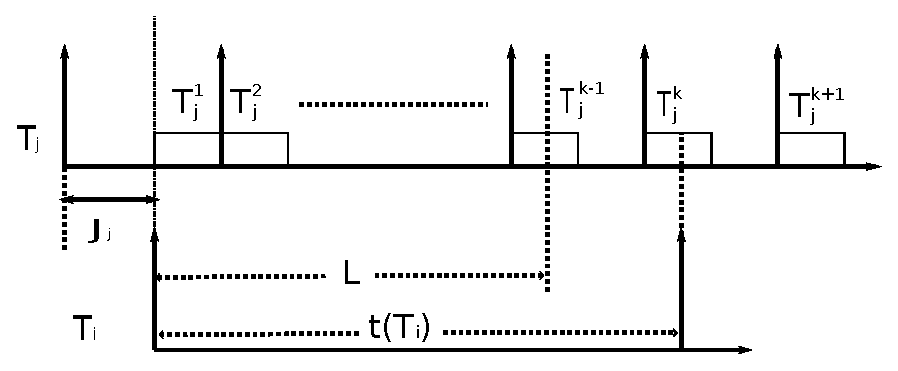
\includegraphics[scale=0.5]{figures/figure11}\caption{\label{fig11}Max interference of $\tau_{j}$ to $\tau_{i}$ in G-RMA}
%%BR: $T_{j}$ and $T_{i}$ are task periods. Is that what you meant here?
\end{figure}

Thus, the maximum contribution of $\tau_{j}^b$ to $\tau_{i}^a$ for any duration
$L$ can be deduced from Figure~\ref{fig11} as $W_{ij}(L)=\left(\left\lceil\frac{L-c_{j}}{T_{j}}\right\rceil+1 \right)c_{j}$,
where $L$ can extend to $T_{i}$. Note the contrast with ECM, where $L$ cannot be extended directly to $T_i$, as this will have a different pattern of worst case interference from other tasks.

\subsection{Retry Cost of Atomic Sections}

\begin{clm}
Under RCM, a task $\tau_i$'s retry cost over duration $L$, which can extend to $T_i$, is upper bounded by:
\begin{eqnarray}
RC\left(L\right) & \le & \sum_{\theta\in\theta_{i}}\Bigg(\left(\sum_{\tau_{j}^{*}}\left(\left(\left\lceil\frac{L-c_{j}}{T_{j}}\right\rceil+1\right)\pi\left(j,\theta\right)\right)\right)\nonumber \\
 & - & s_{max}^{min}\left(\theta\right)+s_{i_{max}}\left(\theta\right)\Bigg)\label{eq20}\end{eqnarray}
 where:
 \begin{itemize}
\item $\tau_{j}^{*}=\{\tau_{j}|(\tau_{j}\in\gamma_i(\theta))\wedge(p_{j}> p_{i})\}$
\item $\pi(j,\theta)=\sum_{\forall s_{j}^{l}(\theta)}len\left(s_{j}^{l}\left(\theta\right)+s_{max}^{j}\left(\theta\right)\right)$
\item $s_{max}^{min}(\theta)=min_{\forall \tau_j^*} \{s_{max}^j(\theta)\}$
\end{itemize}
\end{clm}
\begin{proof}
The worst case interference pattern for RCM is the same as that for ECM for an interval $L$, except that, in RCM, $L$ can extend to the entire $T_i$, but in ECM, it cannot, as the interference pattern of $\tau_j$ to $\tau_i$ changes. 
Thus, (\ref{eq16}) can be used to calculate $\tau_i$'s retry cost, with some modifications, as we do not have to obtain the minimum of the two terms in (\ref{eq16}), because $\tau_j$'s atomic sections will abort and retry only atomic sections of tasks with lower priority than $\tau_j$. Thus, $s_{max}(\theta)$, $s_{max}^*(\theta)$, and $\bar{s}_{max}(\theta)$ are replaced by $s_{max}^{min}(\theta)$, which is the minimum of the set of maximum-length atomic sections of tasks with priority lower than $\tau_j$ and share object $\theta$ with $\tau_i$. This is because, the maximum length atomic section of tasks other than $\tau_j$ differs according to $j$. Besides, as $\tau_i$'s atomic sections can be aborted only by atomic sections of higher priority tasks, not all $\tau_j \in \gamma (\theta)$ are considered, but only the subset of tasks in $\gamma (\theta)$ with priority higher than $\tau_i$ (i.e., $\tau_j^*$). 
Claim follows.
\end{proof}



\subsection{Upper Bound on Response Time}

The response time upper bound can be computed using Theorem 7 in~\cite{key-2} with a modification to include the effect of retry cost. The upper bound is given by:
\begin{equation}
R_{i}^{up}=c_{i}+RC(R_{i}^{up})+\left\lfloor\frac{1}{m}\sum_{j\ne i}W_{ij}(R_{i}^{up})\right\rfloor\label{eq22}\end{equation}
where $W_{ij}(R_{i}^{up})$ is calculated as in (\ref{eq14}), $c_{ji}$ is calculated by (\ref{eq9}), and $RC$ is calculated by (\ref{eq20}).

%%BR: Skipped reviewing the following %%%%%%%%%%%%%
\begin{comment}
\section{FMLP and OMLP Blocking Times}
\label{sec:blocking-bound-fmlp-omlp}

The FMLP protocol~\cite{brandenburg2008comparison} has been shown to be superior to other multiprocessor real-time locking protocols in terms of schedulability, and the global OMLP protocol~\cite{key-3} has been shown to be asymptotically optimal. To formally compare STM against FMLP and global OMLP, we first upper bound their blocking times. %(those were not presented in~\cite{brandenburg2008comparison,key-4,key-3}). 


\subsection{\label{global-fmlp}Global FMLP}

FMLP can be used with global and partitioned scheduling. Since we only consider global scheduling, ``FMLP" and ``global FMLP" mean the same, for the paper's purpose.


FMLP divides shared objects into short resources, $s\_\theta$, and long ones, $l\_\theta$. Nested resources 
are grouped together into two groups: $g(s\_\theta)$ that contains only short resources, and $g(l\_\theta)$ that contains only long resources.
A request $R_i (g(s\_\theta))$ is made by a task $T_i$ to access one or more resources in $g(s\_\theta)$. This request's length is denoted $|R_i (g(s\_\theta))|$, and the number of times $T_i$ requests short resources is denoted $N_{i,s}$. Similarly, $R_i (g(l\_\theta))$ is $T_i$'s request to a group containing long resources for a duration $|R_i (g(l\_\theta))|$, and $N_{i,l}$ is the number of times $T_i$ requests long resources.


Global FMLP uses a variant of G-EDF (called GSN-EDF which discriminates between
linked jobs and scheduled ones) to account for non-preemptive jobs while still using G-EDF for scheduling, 
%%BR: "jobs"?? (can there be multiple linked jobs)?
%%BR: "ones"?? (can there be multiple scheduled ones)?
Tasks busy-wait on short resources, and suspend on long ones. In both cases, requests for resources are arranged in FIFO queues, 
%%BR: "FIFO queue" or "FIFO queues"???? (since there are two resource types)
and for requesting long resources, the task holding the resource inherits the highest priority of the suspended tasks on that resource. For short resources, there is no need to inherit priorities, as tasks become non-preemptable when acquiring short resources. 

Requests for long resources can contain requests for the short resource group, but the reverse is not true. The protocol allows non-preemptable jobs and bounds the time a job is non-preemptively blocked by a lower priority job as the maximum time a non-preemptive section of the job can be linked to the processor of the higher priority job. This non-preemptive blocking can only happen when the higher priority job is released or resumed.


Three types of blocking can be incurred by any task under global FMLP. These include busy-wait blocking, non-preemptive blocking, and direct blocking. The total blocking time of a job, $b_{i}$, is the sum of these three blocking durations. Execution time of each task, $e_{i}$, is inflated by this blocking amount ($e_{i}+b_{i}$), and is used in any of the G-EDF schedulability tests (e.g.,~\cite{Goossens:2003:PSP:876600.876615,srinivasan2002deadline}) 
for verifying schedulability. 

We upper bound a task's blocking durations due to busy-wait blocking, non-preemptive blocking, and direct blocking, denoted as $BW(T_{i})$, $NPB(T_{i})$, and $DB(T_{i})$, respectively, as follows.  
(Note that, in~\cite{key-3}, no upper bounds are presented for these terms, except for $DB(T_{i})$, as~\cite{key-3}'s main focus is on FMLP's suspension-based part. Also, the upper bound for $DB(T_{i})$ in~\cite{key-3} does not consider the effect of requesting a short resource within a long one.)


A job $T_{i}^{j}$ busy-waits in a FIFO queue when it is scheduled on a processor and it cannot be removed by any other task until its request is satisfied. As busy-waiting tasks are non-preemptable, job $T_{i}^{j}$ can be blocked for at most the maximum $m-1$ requests, where each request consists of the sum of the nested requests
to some resources in the same group. This process proceeds for each short resource requested by $T_{i}$. The busy-wait blocking time, $BW(T_{i})$, is therefore:
\begin{equation}
BW(T_{i})\le\sum_{s\_\theta\in\theta_{i}} \left(max \left[\sum_{k=1,k\ne i}^{min(m,n)-1} \left| R_{k} \left(g \left(s\_\theta \right) \right) \right| \right] \right)\label{eq26}
\end{equation}

A job $T_{i}^{j}$ can be non-preemptively blocked, either at its release or when it resumes, by at most the maximum (nested) request to any short resource. The non-preemptive blocking time, $NPB(T_{i})$, is therefore:
\begin{equation}
NPB(T_{i})=(1+N_{i,l}).max_{k\ne i} \left| R_{k}(g(s\_\theta)) \right|\label{eq27}
\end{equation}
Here, $1$ is added to $N_{i,l}$, because $T_{i}$ can be non-preemptively blocked at its release, in addition to suspension times. 

A job $T_{i}^{j}$ can be blocked by all other $n-1$ tasks for any long resource. Any of these $n-1$ requests can be a nested request to long resources belonging to the same group. In addition, any of those requests can contain a request to a short resource, and so it can busy-wait on it. Thus, each request in the $n-1$ requests, requiring access to a short resource, can be delayed by at most the maximum $m-1$ requests to the group containing that short resource. The direct blocking time, $DB(T_{i})$, is therefore:
\begin{equation}
DB(T_{i})\le\sum_{l\_\theta\in\theta_{i}} \left[max_{k=1,k\ne i}^{n-1} \left|R_{k} \left(g \left(l\_\theta \right) \right) \right| \right]
\label{eq28}
\end{equation}


\subsection{Global OMLP}


In~\cite{key-3}, 
global FMLP has a maximum s-oblivious pi-blocking cost of $\Theta(n)$, whereas global OMLP~\cite{key-3}, which is a suspension-based protocol that supports G-EDF, as well as any global job-level static priority (JLSP) scheduler, has a $\Theta(m)$ s-oblivious pi-blocking cost, as seen by equation (\ref{eq29}):
\begin{equation}
b_{i}\triangleq\sum_{k=1}^{q}N_{i,k}.2.(m-1).max_{1\le i\le n}\{L_{i,k}\}\label{eq29}\end{equation}
where $N_{i,k}$ is the maximum number of times $T_i$ requests resource $k$, and $L_{i,k}$ is the maximum execution time of such a request. $N_{i,k}$ and $L_{i,k}$ are assumed to be constants,
so the s-oblivious pi-blocking is $\Theta(m)$, and thus it is optimal.
\end{comment}

%%BR: Resumed editing from here
\section{STM versus Lock-Free}
\label{sec:comparison}

We now would like to understand when STM will be beneficial compared to lock-free synchronization. The retry-loop lock-free approach in~\cite{key-5} is the most relevant to our work. 


\subsection{\label{sub:G-EDF-scheduler-with} ECM versus Lock-Free}

\begin{clm}
For ECM's schedulability to be better or equal to that of~\cite{key-5}'s retry-loop lock-free approach,  
the size of $s_{max}$ must not exceed one half of that of $r_{max}$, where $r_{max}$ is the maximum execution cost of a single iteration of any lock-free retry loop of any task. With low number of conflicting tasks, the size of $s_{max}$ can be at most the size of $r_{max}$. 
\end{clm}
\begin{proof}
Equation (\ref{eq17}) can be upper bounded as:
\begin{equation}
RC\left(T_{i}\right) \le \sum_{\tau_{j}\in\gamma_{i}}\left(\sum_{\theta\in\theta_{i}}\left(\left\lceil\frac{T_{i}}{T_{j}}\right\rceil\sum_{\forall s_{j}^{l}\left(\theta\right)}\left(2.s_{max}\right)\right)\right)
\label{eq30}
\end{equation}
where $s_{j}^{l}\left(\theta\right)$, $s_{i_{max}}\left(\theta\right)$,
$s_{max}^{*}\left(\theta\right)$, and $\bar{s}_{max}\left(\theta\right)$ are replaced by $s_{max}$, and the order of the first two summations are reversed
by each other, 
with $\gamma_{i}$ being the set of tasks that share objects
with $\tau_{i}$. These changes are done to simplify the comparison.

Let $\sum_{\theta\in\theta_{i}}\sum_{\forall s_{j}^{l}\left(\theta\right)}=\beta_{i,j}^{*}$, and $\alpha_{edf}=\sum_{\tau_{j}\in\gamma_{i}}\left\lceil\frac{T_{i}}{T_{j}}\right\rceil.2\beta_{i,j}^*$. Now, (\ref{eq30}) can be modified as:
\begin{equation}
RC\left(T_{i}\right)=\alpha_{edf}.s_{max}
\label{eq31}
\end{equation}

The loop retry cost is given by:
\begin{eqnarray}
LRC\left(T_i\right)&=&\sum_{\tau_{j}\in\gamma_{i}}\left(\left\lceil\frac{T_{i}}{T_{j}}\right\rceil+1\right).\beta_{i,j}.r_{max}\nonumber \\
&=& \alpha_{free} . r_{max} \label{eq32}
\end{eqnarray}
where $\beta_{i,j}$ is the number of retry loops of $\tau_{j}$ that accesses the same object as that accessed by some retry loop of $\tau_{i}$, and $\alpha_{free} = \sum_{\tau_{j}\in\gamma_{i}}\left(\left\lceil\frac{T_{i}}{T_{j}}\right\rceil + 1 \right).\beta_{i,j}$.
Since the shared objects are the same in both STM and lock free, $\beta_{i,j}=\beta_{i,j}^{*}$.
Thus, STM achieves equal or better schedulability 
than lock-free if the total utilization of the STM system is less than or equal to that of the lock-free system:
\begin{eqnarray}
\sum_{\tau_{i}}\frac{c_{i}+\alpha_{edf}.s_{max}} {T_{i}} & \le & \sum_{\tau_{i}}\frac{c_{i}+\alpha_{free}.r_{max}}{T_{i}} \nonumber \\
\therefore\frac{s_{max}}{r_{max}} & \le & \frac{\sum_{\tau_{i}}\alpha_{free}/T_{i}}{\sum_{\tau_{i}}\alpha_{edf}/T_{i}}\end{eqnarray}


Let $\bar{\alpha}_{free}=\sum_{\tau_{j}\in\gamma_{i}}\left\lceil\frac{T_{i}}{T_{j}}\right\rceil.\beta_{i,j}$,  $\hat{\alpha}_{free}=\sum_{T_{j}\in\gamma_{i}}\beta_{i,j}$, and $\alpha_{free}=\bar{\alpha}_{free}+\hat{\alpha}_{free}.$ Therefore: 
\begin{eqnarray}
\frac{s_{max}}{r_{max}} & \le & \frac{\sum_{\tau_{i}}(\bar{\alpha}_{free} +\hat{\alpha}_{free})/T_{i}}{\sum_{\tau_{i}}\alpha_{edf}/T_{i}}\nonumber \\
 & = & \frac{1}{2}+\frac{\sum_{\tau_{i}}\hat{\alpha}_{free} /T_{i}}{\sum_{\tau_{i}}\alpha_{edf}/T_{i}}
 \label{eq33}
 \end{eqnarray}

Let $\zeta_{1}=\sum_{\tau_{i}}\hat{\alpha}_{free}/T_{i}$
and $\zeta_{2}=\sum_{\tau_{i}}\left(\frac{\alpha_{edf}}{2}\right)/T_{i}$. The maximum value of $\frac{\zeta_{1}}{2.\zeta_{2}}=\frac{1}{2}$, which can happen if $T_{j}\ge T_{i}\,\therefore\left\lceil\frac{T_{i}}{T_{j}}\right\rceil=1$. Then $(\ref{eq33})=1$, which is its maximum value. $T_{j}\ge T_{i}$ means that there is a small number of interferences from other tasks
to $\tau_{i}$, and thus low number of conflicts. Therefore, $s_{max}$ is
allowed to be as large as $r_{max}$.

The theoretical minimum value for $\frac{\zeta_{1}}{2.\zeta_{2}}$
is $0$, which can be asymptotically reached if $T_{j}\ll T_{i}$,
$\therefore\,\left\lceil\frac{T_{i}}{T_{j}}\right\rceil\rightarrow\infty$
and $\zeta_{2}\rightarrow\infty$. Thus, $(\ref{eq33})\rightarrow1/2$.

$\beta_{i,j}$ has little effect on $s_{max}/r_{max}$, 
as it is contained in both the numerator and denominator. Irrespective of whether $\beta_{i,j}$ is going to reach its maximum or minimum value, both can be considered constants, and thus removed from (\ref{eq33})'s numerator and denominator. 
However, the number of
interferences of other tasks to $\tau_{i}$, $\left\lceil\frac{T_{i}}{T_{j}}\right\rceil$,
has the main effect on $s_{max}/r_{max}$. This is illustrated in Figure~\ref{fig14}. Claim follows.
\end{proof}

\begin{figure}
\begin{centering}
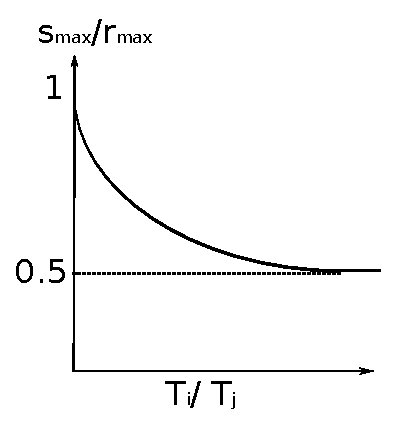
\includegraphics[scale=0.5]{figures/figure14}
\par\end{centering}
\caption{\label{fig14}Effect of $\left\lceil\frac{T_{i}}{T_{j}}\right\rceil$ on
$\frac{s_{max}}{r_{max}}$}
\end{figure}

%%BR: Stopped here. 3:32PM, 10/18/11.

\subsection{RCM versus Lock-Free}

\begin{clm}
For RCM's schedulability to be better or equal to that of~\cite{key-5}'s retry-loop lock-free approach, the size of $s_{max}$ must not exceed one half of that of $r_{max}$ for all cases.
However, the size of $s_{max}$ can be larger than that of $r_{max}$, depending on the number of accesses to a task $T_i$'s shared objects from other tasks.
\end{clm}
\begin{proof}
Equation (\ref{eq20}) is upper bounded by:
 \begin{equation}
\sum_{\left(\tau_{j}\in\gamma_{i}\right)\wedge\left(p_{j}> p_{i}\right)}\left(\left\lceil\frac{T_{i}-c_{j}}{T_{j}}\right\rceil+1\right).2.\beta_{i,j}.s_{max}
\label{eq34}\end{equation}

Consider the same assumptions as in Section~\ref{sub:G-EDF-scheduler-with}.
Let $\alpha_{rma}=\sum_{\left(\tau_{j}\in\gamma_{i}\right)\wedge\left(p_{j}> p_{i}\right)}\left(\left\lceil\frac{T_{i}-c_{j}}{T_{j}}\right\rceil+1\right).2.\beta_{i,j}$. Now, the ratio $s_{max}/r_{max}$ is upper bounded by:
\begin{equation}
\frac{s_{max}}{r_{max}}\le\frac{\sum_{T_{i}}\alpha_{free}/t\left(T_{i}\right)}{\sum_{T_{i}}\alpha_{rma}/t\left(T_{i}\right)}
\label{eq35}\end{equation}

The main difference between RCM and lock-free is that RCM is affected only by the higher priority tasks, while lock-free is affected by all tasks (just as in ECM). 
Besides, RCM
is still affected by $2.\beta_{i,j}$ (just as in ECM).
The subtraction of $c_{j}$ in the numerator of (\ref{eq34}) may not
have a significant effect on the ratio of (\ref{eq35}), as the loop retry 
cost can also be modified to account for the effect of the first interfering
instance of task $T_{j}$. Therefore, 
$\alpha_{free} = \sum_{\tau_{j}\in\gamma_{i}}\left(\left\lceil\frac{T_{i}-c_j}{T_{j}}\right\rceil + 1 \right)\beta_{i,j}$.

Let tasks in the denominator of (\ref{eq35}) be given indexes $k$ instead of $i$, and $l$ instead of $j$. Let tasks in both the numerator and denominator of (\ref{eq35}) be arranged in the non-increasing priority order, so that $i=k$ and $j=l$. Let $\alpha_{free}$ in (\ref{eq35}) be divided into two parts: $\bar{\alpha}_{free}$ that contains only tasks with priority higher than $\tau_i$, and $\hat{\alpha}_{free}$ that contains only tasks with priority lower than $\tau_i$. Now, (\ref{eq35}) becomes:
\begin{eqnarray}
\frac{s_{max}}{r_{max}} & \le & \frac{\sum_{\tau_{i}}(\bar{\alpha}_{free}+\hat{\alpha}_{free})/T_{i}}{\sum_{\tau_{k}}\alpha_{rma}/T_{k}}\nonumber \\
 & = & \frac{1}{2}+\frac{\sum_{\tau_{i}}\hat{\alpha}_{free}/T_{i}}{\sum_{\tau_{k}}\alpha_{rma}/T_{k}}\label{eq36}\end{eqnarray}

For convenience, we introduce the following notations:
\begin{eqnarray}
\zeta_{1}& = & \sum_{\tau_{i}}\frac{\sum_{\left(\tau_{j}\in\gamma_{i}\right)\wedge\left(p_{j}<p_{i}\right)}\left(\left\lceil\frac{T_{i}-c_{j}}{T_{j}}\right\rceil+1\right)\beta_{i,j}}{T_{i}}\nonumber\\
& = & \sum_{T_i} \hat{\alpha}_{free}/T_i
\nonumber\\
\zeta_{2} 
& = & \sum_{\tau_{k}}\frac{\sum_{\left(\tau_{l}\in\gamma_{k}\right)\wedge\left(p_{l}>p_{k}\right)}\left(\left\lceil\frac{T_{k}-c_{l}}{T_{l}}\right\rceil+1\right)\beta_{k,l}}{T_{k}}\nonumber\\
& = & \frac{1}{2}\sum_{\tau_k} \alpha_{rma}/T_k\nonumber
\end{eqnarray}
$\tau_{j}$ is of lower priority than $\tau_{i}$, which means $D_{j}>D_{i}$. Under G-RMA, this means, $T_{j}>T_{i}$.
Thus, $\left\lceil\frac{T_{i}-c_{j}}{T_{j}}\right\rceil=1$ for
all $\tau_{j}$ and $\zeta_{1}=\sum_{\tau_{i}}(\sum_{(\tau_{j}\in\gamma_{i})\wedge(p_{j}<p_{i})}(2.\beta_{i,j}))/T_{i}$.
Since $\zeta_{1}$ contains all $\tau_{j}$ of lower priority than
$\tau_{i}$ and $\zeta_{2}$ contains all $\tau_{l}$ of higher priority than $\tau_{k}$, 
and tasks are arranged in the non-increasing priority order, then for each $\tau_{i,j}$, there exists $\tau_{k,l}$ such
that $i=l$ and $j=k$. Figure~\ref{fig:matrix-example} illustrates this, where 0 means that the pair $i,j$ 
does not exist in $\zeta_{1}$,
and the pair $k,l$ does not exist in $\zeta_{2}$' (i.e., 
there is no task $\tau_l$ that will interfere with $\tau_k$ in $\zeta_2$), 
and 1 means the opposite. 

\begin{figure}[htbp]
\begin{tabular}{ccc}
$\begin{array}{cccccc}
 & j & 1 & 2 & \cdots & n\\
i\\
1 &  & 0 & 1 & \cdots & 1\\
2 &  & 0 & 0 & \ddots & \vdots\\
\vdots &  & \vdots & \vdots & \ddots & 1\\
n &  & 0 & 0 & \cdots & 0\end{array}$ &  & $\begin{array}{cccccc}
 & l & 1 & 2 & \cdots & n\\
k\\
1 &  & 0 & 0 & \cdots & 0\\
2 &  & 1 & 0 &  & \vdots\\
\vdots &  & \vdots & \ddots & \ddots & 0\\
n &  & 1 & \cdots & 1 & 0\end{array}$\tabularnewline
\end{tabular}
\caption{\label{fig:matrix-example} Task association for lower priority tasks than $T_i$ and higher priority tasks than $T_k$}
\end{figure}


Thus, it can be seen that both the matrices are transposes of
each other. Consequently, for each $\beta_{i,j}$, there exists $\beta_{k,l}$
such that $i=l$ and $j=k$. But the number of times $\tau_{j}$ accesses
a shared object with $\tau_{i}$ may not be the same as the number of times
$\tau_{i}$ accesses that same object. Thus, $\beta_{i,j}$ does not have
to be the same as $\beta_{k,l}$, even if $i,j$ and $k,l$ are transposes 
of each other. Therefore, we can analyze the behavior of $s_{max}/r_{max}$ based on the three parameters $\beta_{i,j}$, $\beta_{k,l}$, and $\left\lceil\frac{T_{k}-c_{l}}{T_{l}}\right\rceil$.
If $\beta_{i,j}$ is increased so that $\beta_{i,j}\rightarrow\infty$,
$\therefore\,(\ref{eq36})\rightarrow\infty$.
This is because, $\beta_{i,j}$ represents the number of times a lower priority task $\tau_{j}$ accesses 
shared objects with a higher priority task $\tau_{i}$. 
While this number has a greater effect in lock-free, it does not have any effect under RCM, because lower priority tasks do not affect higher priority
ones. Hence, $s_{max}$ is allowed to be much greater than $r_{max}$.

Although the minimum value for $\beta_{i,j}$ is 1, mathematically, if $\beta_{i,j}\rightarrow0$, then (\ref{eq36}) 
 $\rightarrow1/2$.
Here, changing $\beta_{i,j}$ does not affect the retry cost of RCM, but it does affect the retry cost of lock-free, because the contention between tasks is reduced. Thus, $s_{max}$ is reduced in this case to
a little more than half of $r_{max}$ (``a little more''
because the minimum value of $\beta_{i,j}$ is actually 1, not 0).


The change of $s_{max}/r_{max}$ with respect to $\beta_{i,j}$ is illustrated in Figure~\ref{fig15-a}.
If $\beta_{k,l}\rightarrow\infty$, then (\ref{eq36}) $\rightarrow1/2$.
This is because, $\beta_{k,l}$ represents the number of times 
a higher priority task $\tau_{l}$ accesses shared objects with a lower
priority task $\tau_{k}$. Under RCM, this will increase the retry 
cost, thus reducing $s_{max}/r_{max}$. But if $\beta_{k,l}\rightarrow0$, then (\ref{eq36})$\rightarrow\infty$. This is due to the lower contention from a higher priority task $\tau_{l}$ to a lower priority task $\tau_{k}$, which reduces the retry cost under RCM and allows $s_{max}$ to be very large compared with $r_{max}$. Of course, the actual minimum value for $\beta_{k,l}$ is 1, and is illustrated in Figure~\ref{fig15-b}.

%%%%%%

The third parameter that affects $s_{max}/r_{max}$ is $T_{k}/T_{l}$.
If $T_{l}\ll T_{k}$, then $\left\lceil\frac{T_{k}-c_{l}}{T_{l}}\right\rceil\rightarrow\infty$,
and (\ref{eq36}) $\rightarrow1/2$. This is due to a high number
of interferences from a higher priority task $\tau_{l}$ to a lower priority
task $\tau_{k}$, which increases the retry cost under RCM, 
%%BR: WHy don't you say "RCM"? Fix it. 
and consequently reduces $s_{max}/r_{max}$. 

If $T_{l}=T_{k}$ (which is
the maximum value for $T_{l}$ as $D_{l}\le D_{k}$, because
$\tau_{l}$ has a higher priority than $\tau_{k}$), then $\left\lceil\frac{T_{k}-c_{l}}{T_{l}}\right\rceil\rightarrow1$
and $\zeta_2=\sum_{\tau_{k}}\frac{\sum_{\left(\tau_{l}\in\gamma_{k}\right)\wedge\left(p_{l}>p_{k}\right)}2\beta_{k,l}}{t_{k}}$. 
This means that the system will be controlled by only two parameters, $\beta_{i,j}$ and $\beta_{k,l}$, as in the previous two cases, illustrated in Figures~\ref{fig15-a} and~\ref{fig15-b}. Claim follows.
\end{proof}

\begin{figure}
\begin{centering}
\subfigure[\label{fig15-a}]{\begin{centering}
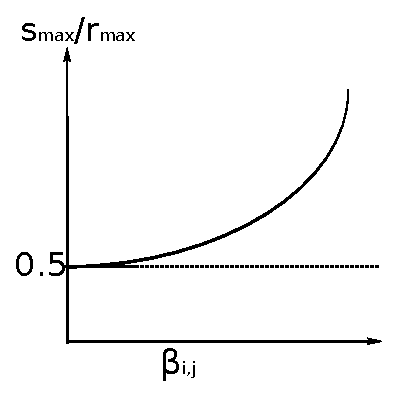
\includegraphics[scale=0.5]{figures/figure15-a}
\par\end{centering}
}\subfigure[\label{fig15-b}]{\begin{centering}
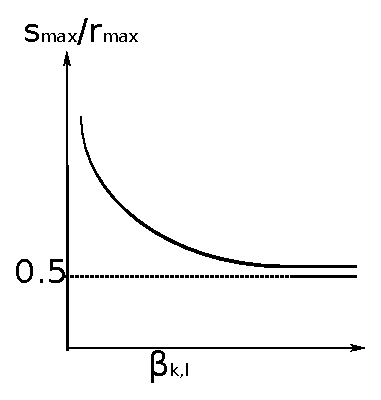
\includegraphics[scale=0.5]{figures/figure15-b}
\par\end{centering}
}
\par\end{centering}
\centering{}\caption{\label{fig15} Change of $s_{max}/r_{max}$: a) $\frac{s_{max}}{r_{max}}$
versus $\beta_{i,j}$ and b) $\frac{s_{max}}{r_{max}}$ versus $\beta_{k,l}$}
\end{figure}


%%BR: Skipped editing from here......
\begin{comment}
\subsection{FMLP \& OMLP versus ECM and RCM
}

\begin{clm}
For ECM's schedulability to be better or equal to that of FMLP or OMLP, 
$s_{max}/|s\_\theta|_{max}$ (in case of FMLP), where $|s\_\theta|_{max}$ be the maximum short request by any task, and $s_{max}/L_{max}$ (in case of OMLP) must  not exceed $O(\frac{m}{n})$, where $L_{max}=max_{\forall i,\forall k}L_{i,k}$. For RCM's schedulability  
to be better or equal  
to that of OMLP, $s_{max}/L_{max}$ must not exceed $O(\frac{m}{n})$.
\end{clm}
\begin{proof}
As FMLP is used with G-EDF (GSN-EDF), we compare only ECM 
against it. 
%%BR: "...we compare only ECM against it."??? 
First, we derive upper bounds for the blocking parameters of FMLP. When requests are non-nested, each resource (short or long) will be contained in its own group. Let $N_{i,s}$ be the number of times a task $T_{i}$ requests a short
resource, $|s\_\theta|_{i,max}$ be the maximum request for a
short resource by $T_{i}$, $\alpha_{bw}=N_{i,s}.(m-1)$. Now, FMLP's three  blocking terms, described in Section~\ref{global-fmlp}, are upper bounded as follows:
\begin{eqnarray*}
BW(T_{i}) & \le & \sum_{s\_\theta\in\theta_{i}}(m-1).|s\_\theta|_{i,max}\\
 & = & N_{i,s}.(m-1).|s\_\theta|_{i,max}\\
 & \le & N_{i,s}.(m-1).|s\_\theta|_{max}\\
& = & \alpha_{bw}.|s\_\theta|_{max}
 \end{eqnarray*}
\begin{eqnarray*}
NPB\left(T_{i}\right) & \le & \left(1+N_{i,l}\right).max\left(BW_{k\ne i}\left(T_{k}\right)+|s\_\theta|_{k,max}\right)\\
 & \le & \left(1+N_{i,l}\right).max\left(BW_{k\ne i}\left(T_{k}\right)+|s\_\theta|_{max}\right)\\
 & = & \left(1+N_{i,l}\right).|s\_\theta|_{max}.max_{k\ne i}\left(N_{k,s}.\left(m-1\right)+1\right)\\
 & = & \alpha_{npb}.|s\_\theta|_{max}
 \end{eqnarray*}
 where $\alpha_{npb}=\left(1+N_{i,l}\right).max_{k\ne i}\left(N_{k,s}.\left(m-1\right)+1\right)$.
\begin{eqnarray*}
DB\left(T_{i}\right) & \le & N_{i,l}.\left(n-1\right).|l\_\theta|_{i,max}\\
 & \le & N_{i,l}.\left(n-1\right).|l\_\theta|_{max}\\
 \end{eqnarray*}
If $|l\_\theta|_{max}\le c1.|s\_\theta|_{max}$, where $c1$ is the
minimum constant that satisfies this relation, then
\begin{eqnarray*}
DB\left(T_{i}\right)& \le & N_{i,l}.\left(n-1\right).c1.|s\_\theta|_{max}\\
& = & \alpha_{db}.|s\_\theta|_{max}
\end{eqnarray*}
where $\alpha_{db}=N_{i,l}.\left(n-1\right).c1$. 

The total blocking time of each task is added to the task execution time, and
as before, we compare the total utilization of the G-EDF system (with both contention managers) against that under FMLP. 

Now, for ECM's schedulability to be better than FMLP,
\begin{equation}
 \frac{s_{max}}{|s\_\theta|_{max}}\le
 \frac{\sum_{T_{i}}\left(\alpha_{bw}+\alpha_{npb}+\alpha_{db}\right) \Big/t(T_{i})}{\sum_{T_{i}}\alpha_{edf} \Big/t(T_{i})}
 \label{eq38} \end{equation}

From (\ref{eq38}), it can be seen that $T_{i}$'s blocking time,
under FMLP, depends on $m,\, n$ and the number of times it requests resources
(in contrast to ECM, 
%%BR: "...contrast to ECM,..."???  
under which, $T_i$'s retry cost depends on the number of times a conflicting task $T_{j}$ requests resources). Thus, if $N_{i,s},\, N_{i,l}$, 
and $N_{k,s}$ can all be upper bounded by some constant $C_{2}$,
which is the maximum number of times any task $T_{i}$ can request a short
or long resource, then the numerator in (\ref{eq38}) 
is $O(n(n+m))$, while the denominator is $O(n^{2})$. Therefore:
\begin{equation}
\frac{s_{max}}{|s\_\theta|_{max}}=O\left(\frac{m}{n} \right)
\label{eq45}
\end{equation}
This means that, for $n<m$, the contention between tasks under both STM and
FMLP is low (even for short resources under FMLP), but FMLP is more affected
by $NTB$. When $n>m$, contention increases, but FMLP arranges
requests in a FIFO queue, so it is less affected than ECM, 
%%BR: "..than ECM,...???
which
suffers from conflicting tasks and instances
of each conflicting one. FMLP is not affected by the number of instances
of each conflicting task.

%%%%
Since OMLP's blocking time is bounded by (\ref{eq29}) \[ \therefore 
%\;
bi\le2.\left(m-1\right).L_{max}\sum_{k=1}^{q}N_{i,k}\]
%%BR: THis sentence is awkward. Why don't you say "Let  \[L_{max}=..... Since OMLP's blocking time is ..., \therefore.."


For ECM's schedulability to be better than global OMLP:
\begin{equation}
\frac{s_{max}}{L_{max}}\le\frac{\sum_{T_{i}}\left(2.\left(m-1\right)\sum_{k=1}^{q}N_{i,k}\right) \Big/t\left(T_{i}\right)}{\sum_{T_{i}}\alpha_{edf} \Big/t\left(T_{i}\right)}\label{eq40}\end{equation}

For RCM, the ratio is:
\begin{equation}
\frac{s_{max}}{L_{max}}\le\frac{\sum_{T_{i}}\left(2.\left(m-1\right)\sum_{k=1}^{q}N_{i,k}\right) \Big/t\left(T_{i}\right)}{\sum_{T_{i}}\alpha_{rma} \big/t\left(T_{i}\right)}\label{eq41}\end{equation}


If $\sum_{k=1}^{q}N_{i,k}$ is upper bounded by $C_{3}$, which is
a constant representing the maximum total number of requests for resources
by any task $T_{i}$, then:
\begin{equation}
\frac{s_{max}}{L_{max}}=O\left(\frac{nm}{n^{2}}\right)=O\left(\frac{m}{n}\right)
\label{eq46}
\end{equation}
for each of (\ref{eq40}) and (\ref{eq41}). Claim follows.
\end{proof}
\end{comment}


%%BR: Re-started editing from here:
\section{Conclusions}
\label{sec:conclusions}

Under both ECM and RCM,  
a task incurs $2.s_{max}$ retry cost for each of its atomic sections due to a conflict with another task's atomic section. Retries under RCM and lock-free are affected by a larger number of conflicting task instances than under ECM. While task retries under ECM and lock-free are affected by all other tasks, retries under RCM are affected only by higher priority tasks. 


STM and lock-free have similar parameters that affect their retry costs---i.e., the number of conflicting jobs and how many times they access shared objects. The $s_{max}/r_{max}$ ratio determines whether STM is better or as good as lock-free. For ECM, this ratio cannot exceed 1, and it can be 1/2 for higher number of conflicting tasks. For RCM, for the common case, $s_{max}$ must be 1/2 of $r_{max}$, and in some cases, $s_{max}$ can be larger than $r_{max}$ by many orders of magnitude.


Our work raises several questions. 
%The questions that we ask (see Section~\ref{sec:intro}) are fundamentally analytical in nature, and hence, our results are analytical. However, significant insights can be gained by experimental work on a broad range of embedded software, which is outside our work's scope. 
For example, what are the typical range of values for the different parameters that affect the retry cost (and hence the response time)? How tight is our retry and response time bounds in practice? Can real-time CMs be designed for other multiprocessor real-time schedulers (e.g., partitioned, semi-partitioned), and those that dynamically improve application timeliness behavior? These are important directions for further work. 

\chapter{LCM}

We consider software transactional memory (STM) concurrency control for multicore real-time software. We present a novel contention manager (CM) for resolving transactional conflicts, called length-based CM (or LCM). We upper bound transactional retries and response times under LCM, when used with G-EDF and  G-RMA schedulers. We identify the conditions under which LCM outperforms previous real-time STM CMs and lock-free synchronization. Our implementation and experimental studies reveal that G-EDF/LCM and G-RMA/LCM have shorter or comparable retry costs and response times than other synchronization techniques.

\section{Length-based CM}

LCM resolves conflicts based on the priority of conflicting jobs, besides the length of the interfering atomic section, and the length of the interfered atomic section. This is in contrast to ECM and RCM~\cite{stmconcurrencycontrol:emsoft11}, where conflicts are resolved using the priority of the conflicting jobs. This strategy allows lower priority jobs, under LCM, to retry for lesser time than that under ECM and RCM, but higher priority jobs, sometimes, wait for lower priority ones with bounded priority-inversion.

\subsection{\label{sec 9.1} Design and Rationale}

%Begin algorithm here
\begin{algorithm}
\footnotesize{
\LinesNumbered
\KwData{$s_i^k(\theta)\rightarrow$ interfered atomic section.\\$s_j^l(\theta)\rightarrow$ interfering atomic section.\\$\psi\rightarrow$ predefined threshold $\in [0,1]$.\\$\delta_i^k(\theta)\rightarrow$ remaining execution length of $s_i^k(\theta)$}
\KwResult{which atomic section of $s_i^k(\theta)$ or $s_j^l(\theta)$ aborts}
\eIf{$p_i^k > p_j^l$}
	{$s_j^l(\theta)$ aborts\label{step_sicommits}\;}
	{$c_{ij}^{kl}=len(s_j^l(\theta))/len(s_i^k(\theta))$\label{step_cijkl}\;
	$\alpha_{ij}^{kl}=ln(\psi)/(ln(\psi)-c_{ij}^{kl})$\label{step_alphaijkl}\;
	$\alpha=\left(len(s_i^k(\theta))-\delta_i^k(\theta)\right)/len(s_i^k(\theta))$\;
	\eIf{$\alpha \le \alpha_{ij}^{kl}$}
	{$s_i^k(\theta)$ aborts\label{step_siaborts}\;}
	{$s_j^l(\theta)$ aborts\label{step_sjaborts}\;}
	}
	}
\caption{LCM}
\label{alg_lcm}
\end{algorithm}
%End algorithm here

For both ECM and RCM, $s_{i}^{k}(\theta)$ can be totally repeated if $s_{j}^{l}(\theta)$ --- which belongs to a higher priority job $\tau_{j}^b$ than $\tau_{i}^a$ --- conflicts with $s_{i}^{k}(\theta)$
at the end of its execution, while $s_{i}^{k}(\theta)$ is just about
to commit. Thus, LCM, shown in Algorithm~\ref{alg_lcm}, uses the remaining length of $s_{i}^{k}(\theta)$ when it is interfered,
as well as $len(s_{j}^{l}(\theta))$, to decide which transaction must be aborted. If $p_i^k$ was greater than $p_j^l$, then $s_i^k(\theta)$ would be the one that commits, because it belongs to a higher priority job, and it started before $s_j^l(\theta)$ (step~\ref{step_sicommits}). Otherwise, $c_{ij}^{kl}$ is calculated (step~\ref{step_cijkl}) to determine whether it is worth aborting $s_i^k(\theta)$ in favor of $s_j^l(\theta)$, because $len(s_j^l(\theta))$ is relatively small compared to the remaining execution length of $s_i^k(\theta)$  (explained further).

We assume that:
\begin{equation}
c_{ij}^{kl}=len(s_{j}^{l}(\theta))/len(s_{i}^{k}(\theta))
\label{cm_eq}\end{equation}
where $c_{ij}^{kl}\in]0,\infty[$, to cover all possible lengths of $s_{j}^{l}(\theta)$.
Our idea is to reduce the opportunity for the abort of $s_{i}^{k}(\theta)$ if it is close to committing when interfered and $len(s_{j}^{l}(\theta))$ is large. This abort opportunity is increasingly reduced as $s_{i}^{k}(\theta)$ gets closer to the end of its execution, or $len(s_{j}^{l}(\theta))$ gets larger. 

On the other hand, as $s_{i}^{k}(\theta)$ is interfered early,
or $len(s_{j}^{l}(\theta))$ is small compared to $s_{i}^{k}(\theta)$'s remaining length, the abort opportunity 
is increased even if $s_i^k (\theta)$ is close to the end of its execution. To decide whether $s_{i}^{k}(\theta)$ must be aborted or not, we use a threshold value $\psi\in[0,1]$ that determines $\alpha_{ij}^{kl}$ (step~\ref{step_alphaijkl}), where $\alpha_{ij}^{kl}$ is the maximum percentage of $len(s_i^k(\theta))$ below which $s_j^l(\theta)$ is allowed to abort $s_i^k(\theta)$. Thus, if the already executed part of $s_i^k(\theta)$ --- when $s_j^l(\theta)$ interferes with $s_i^k(\theta)$ --- does not exceed $\alpha_{ij}^{kl}len(s_i^k(\theta))$, then $s_i^k(\theta)$ is aborted (step~\ref{step_siaborts}). Otherwise, $s_j^l(\theta)$ is aborted (step~\ref{step_sjaborts}).

%
\begin{figure}[htbp]
\centering
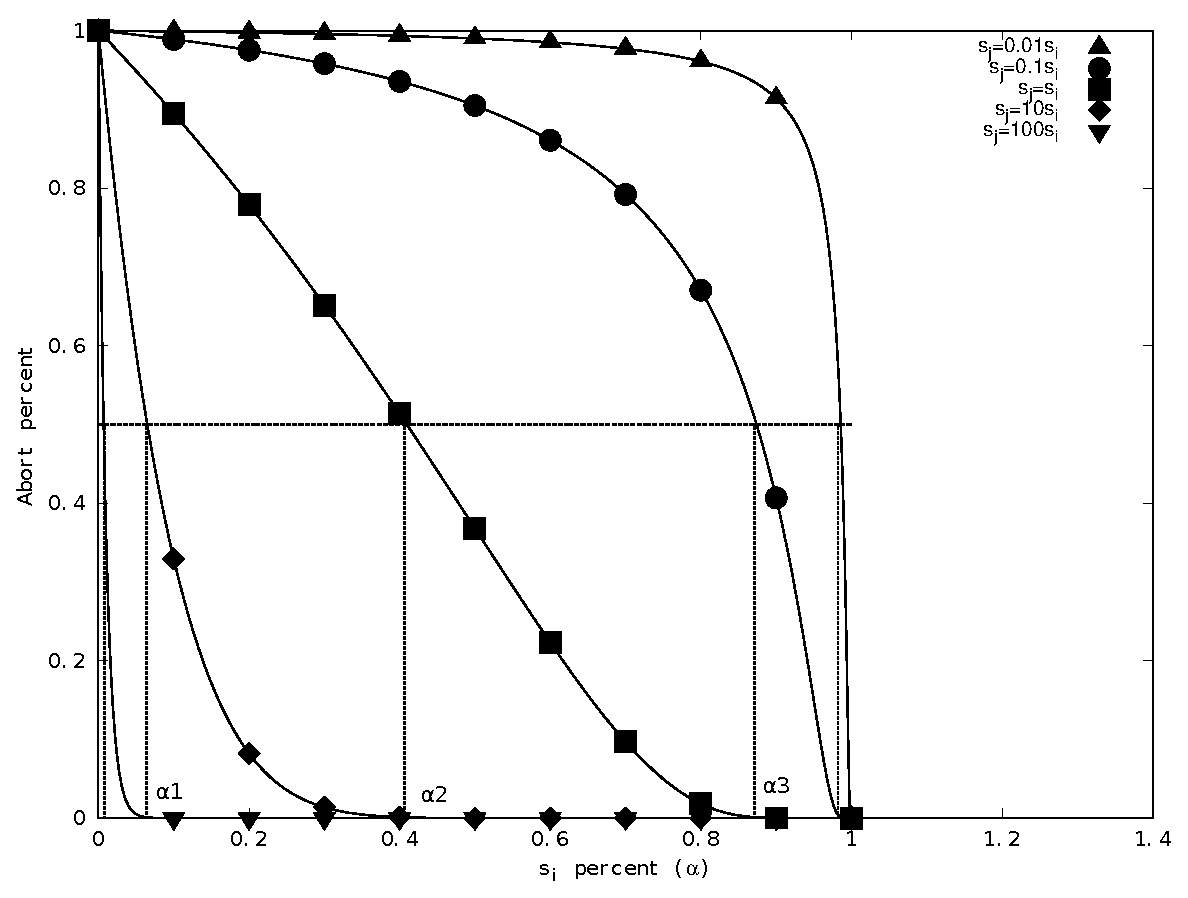
\includegraphics[scale=0.4]{figures/figure16}
\caption{\label{fig16}Interference of $s_{i}^{k}(\theta)$ by various lengths of 
$s_{j}^{l}(\theta)$}
\end{figure}

The behavior of LCM is illustrated in Figure~\ref{fig16}. In this figure, the horizontal axis corresponds to different values of $\alpha$ ranging from $0$ to $1$, and the vertical axis corresponds to different values of abort opportunities, $f(c_{ij}^{kl},\alpha)$, ranging from $0$ to $1$ and calculated by~(\ref{eq49}):
\begin{equation}
f(c_{ij}^{kl},\alpha)=e^{\frac{-c_{ij}^{kl}\alpha}{1-\alpha}}
\label{eq49}\end{equation}
where $c_{ij}^{kl}$ is calculated by~(\ref{cm_eq}).

Figure~\ref{fig16} shows one atomic section $s_i^k(\theta)$ (whose $\alpha$ changes along the horizontal axis) interfered by five different lengths of $s_j^l(\theta)$.
For a predefined value of $f(c_{ij}^{kl},\alpha)$ (denoted as $\psi$ in Algorithm~\ref{alg_lcm}), there corresponds a specific value of $\alpha$ (which is $\alpha_{ij}^{kl}$ in Algorithm~\ref{alg_lcm}) for each curve. For example, when $len(s_j^l(\theta))=0.1 \times len(s_i^k(\theta))$, $s_j^l(\theta)$ aborts $s_i^k(\theta)$ if the latter has not executed more than $\alpha3$ percentage (shown in Figure~\ref{fig16}) of its execution length. As $len(s_{j}^{l}(\theta))$ decreases, the corresponding $\alpha_{ij}^{kl}$ increases (as shown in Figure~\ref{fig16}, $\alpha3>\alpha2>\alpha1$).

Equation (\ref{eq49}) achieves the desired requirement that the abort opportunity is reduced as $s_{i}^{k}(\theta)$ gets
closer to the end of its execution (as $\alpha\rightarrow1,\, f(c_{ij}^{kl},1)\rightarrow0$),
or as the length of the conflicting transaction increases (as $c_{ij}^{kl}\rightarrow\infty,\, f(\infty,\alpha)\rightarrow0$).
Meanwhile, this abort opportunity is increased as $s_{i}^{k}(\theta)$
is interfered closer to its release (as $\alpha\rightarrow0,\, f(c_{ij}^{kl},0)\rightarrow1$),
or as the length of the conflicting transaction decreases (as $c_{ij}^{kl}\rightarrow0,\, f(0,\alpha)\rightarrow1$).

LCM is not a centralized CM, which means that, upon a conflict, each transactions has to decide whether it must commit or abort. 

\begin{clm}
\label{LCM_higher_rc}
Let $s_{j}^{l}(\theta)$ interfere once with $s_{i}^{k}(\theta)$ at $\alpha_{ij}^{kl}$. Then, the maximum contribution of $s_{j}^{l}(\theta)$ to 
$s_{i}^{k}(\theta)$'s 
retry cost is:
\begin{equation}
W_i^k(s_j^l(\theta))\le \alpha_{ij}^{kl}len\Big(s_{i}^{k}(\theta)\Big)+len\Big(s_{j}^{l}(\theta)\Big)\label{eq47}\end{equation}
\end{clm}

\begin{proof}
If $s_{j}^{l}(\theta)$ interferes with $s_{i}^{k}(\theta)$
at a $\Upsilon$ percentage, where $\Upsilon<\alpha_{ij}^{kl}$,
then the retry cost of $s_{i}^{k}(\theta)$ is $\Upsilon len(s_{i}^{k}(\theta))+len(s_{j}^{l}(\theta))$, which is lower than that calculated in (\ref{eq47}). Besides, 
if $s_{j}^{l}(\theta)$ interferes with $s_{i}^{k}(\theta)$ after
$\alpha_{ij}^{kl}$ percentage, then $s_{i}^{k}(\theta)$ will not
abort.
\end{proof}


\begin{clm}
\label{LCM_lower_rc}
An atomic section of a higher priority job, $\tau_{j}^b$, may have to abort and retry due to a lower priority job, $\tau_{i}^a$, if $s_{j}^{l}(\theta)$ interferes
with $s_{i}^{k}(\theta)$ after the $\alpha_{ij}^{kl}$ percentage. $\tau_{j}$'s retry time, due to $s_{i}^{k}(\theta)$ and $s_{j}^{l}(\theta)$,
is upper bounded by:
 \begin{equation}
W_j^l(s_i^k(\theta))\le \Big(1-\alpha_{ij}^{kl}\Big)len\Big(s_{i}^{k}(\theta)\Big)\label{eq48}\end{equation}
\end{clm}

\begin{proof}
It is derived directly from Claim~\ref{LCM_higher_rc}, as $s_j^l(\theta)$ will have to retry for the remaining length of $s_i^k(\theta)$.
\end{proof}

%sh-start
\begin{clm}
\label{no priority inversion in lcm}
A higher priority job, $\tau_i^z$, suffers from priority inversion for at most number of atomic sections in $\tau_i^z$.
\end{clm}

\begin{proof}
Assuming three atomic sections, $s_i^k(\theta)$, $s_j^l(\theta)$ and $s_a^b(\theta)$, where $p_j > p_i$ and $s_j^l(\theta)$ interferes with $s_i^k(\theta)$ after $\alpha_{ij}^{kl}$. Then $s_j^l(\theta)$ will have to abort and retry. At this time, if $s_a^b(\theta)$ interferes with the other two atomic sections, and the LCM decides which transaction to commit based on comparison between each two transactions. So, we have the following cases:-
\begin{itemize}
\item $p_a < p_i < p_j$, then $s_a^b(\theta)$ will not abort any one because it is still in its beginning and it is of the lowest priority. So. $\tau_j$ is not indirectly blocked by $\tau_a$.
\item $p_i<p_a<p_j$ and even if $s_a^b(\theta)$ interferes with $s_i^k(\theta)$ before $\alpha_{ia}^{kb}$, so, $s_a^b(\theta)$ is allowed abort $s_i^k(\theta)$. Comparison between $s_j^l(\theta)$ and $s_a^b(\theta)$ will result in LCM choosing $s_j^l(\theta)$ to commit and abort $s_a^b(\theta)$ because the latter is still beginning, and $\tau_j$ is of higher priority. If $s_a^b(\theta)$ is not allowed to abort $s_i^k(\theta)$, the situation is still the same, because $s_j^l(\theta)$ was already retrying until $s_i^k(\theta)$ finishes.
\item $p_a>p_j>p_i$, then if $s_a^b(\theta)$ is chosen to commit, this is not priority inversion for $\tau_j$ because $\tau_a$ is of higher priority.
\item if $\tau_a$ preempts $\tau_i$, then LCM will compare only between $s_j^l(\theta)$ and $s_a^b(\theta)$. If $p_a<p_j$, then $s_j^l(\theta)$ will commit because of its task's higher priority and $s_a^b(\theta)$ is still at its beginning, otherwise, $s_j^l(\theta)$ will retry, but this will not be priority inversion because $\tau_a$ is already of higher priority than $\tau_j$. If $\tau_a$ does not access any object but it preempts $\tau_i$, then CM will choose $s_j^l(\theta)$ to commit as only already running transactions are competing together.
\end{itemize}
So, by generalizing these cases to any number of conflicting jobs, it is seen that when an atomic section, $s_j^l(\theta)$, of a higher priority job is in conflict with a number of atomic sections belonging to lower priority jobs, $s_j^l(\theta)$ can suffer from priority inversion by only one of them. So, each higher priority job can suffer priority inversion at most its number of atomic section. Claim follows.
\end{proof}

\begin{clm}
\label{max_pri_inv}
The maximum delay suffered by $s_j^l(\theta)$ due to lower priority jobs is caused by the maximum length atomic section accessing object $\theta$, which belongs to a lower priority job than $\tau_j^b$ that owns $s_j^l(\theta)$.
\end{clm}

\begin{proof}
Assume three atomic sections, $s_i^k(\theta)$, $s_j^l(\theta)$, and $s_h^z(\theta)$, where $p_j>p_i$, $p_j>p_h$, and $len(s_i^k(\theta))>len(s_h^z(\theta))$. Now, $\alpha_{ij}^{kl}>\alpha_{hj}^{zl}$ and $c_{ij}^{kl}<c_{hj}^{zl}$. By applying~(\ref{eq48}) to obtain the contribution of $s_i^k(\theta)$ and $s_h^z(\theta)$ to the priority inversion of $s_j^l(\theta)$ and dividing them, we get:
\begin{eqnarray*}
\frac{W_{j}^{l}(s_{i}^{k}(\theta))}{W_{j}^{l}(s_{h}^{z}(\theta))} & = & \frac{\left(1-\alpha_{ij}^{kl}\right)len(s_{i}^{k}(\theta))}{\left(1-\alpha_{hj}^{zl}\right)len(s_{h}^{z}(\theta))}
\end{eqnarray*}
By substitution for $\alpha$s from~(\ref{eq49}):
\begin{eqnarray*}
 & = & \frac{(1-\frac{ln\psi}{ln\psi-c_{ij}^{kl}})len(s_{i}^{k}(\theta))}{(1-\frac{ln\psi}{ln\psi-c_{hj}^{zl}})len(s_{h}^{z}(\theta))}
  =  \frac{(\frac{-c_{ij}^{kl}}{ln\psi-c_{ij}^{kl}})len(s_{i}^{k}(\theta))}{(\frac{-c_{hj}^{zl}}{ln\psi-c_{hj}^{zl}})len(s_{h}^{z}(\theta))}\end{eqnarray*}
$\because ln\psi \le 0$ and $c_{ij}^{kl},c_{hj}^{kl} > 0, \therefore$ by substitution from~(\ref{cm_eq})
\begin{eqnarray*}
 & = & \frac{len(s_{j}^{l}(\theta))/(ln\psi-c_{ij}^{kl})}{len(s_{j}^{l}(\theta))/(ln\psi-c_{hj}^{zl})}
  =  \frac{ln\psi-c_{hj}^{zl}}{ln\psi-c_{ij}^{kl}}>1\end{eqnarray*}
Thus, as the length of the interfered atomic section increases, the delay suffered by the interfering atomic section increases. Claim follows.
\end{proof}


\subsection{\label{response g-edf/lcm} Response Time of G-EDF/LCM}

%Toward establishing the response time under G-EDF/LCM, we introduce a set of Claims.

\begin{clm}\label{GEDF/LCM response time}
$RC(T_i)$ for a task $\tau_i$ under G-EDF/LCM is upper bounded by:
\begin{eqnarray}
RC(T_i) & = & \Bigg(\sum_{\forall \tau_h \in \gamma_i}\sum_{\forall\theta \in \theta_i \wedge \theta_h}\Bigg(\left\lceil\frac{T_{i}}{T_{h}}\right\rceil\sum_{\forall s_{h}^{l}(\theta)}len\Big(s_{h}^{l}(\theta)\Big)\nonumber\\
& + & \alpha_{max}^{hl}len\Big(s_{max}^{h}(\theta)\Big)\Bigg)\Bigg)\nonumber\\
& + & \sum_{\forall s_{i}^{y}(\theta)}\Big(1-\alpha_{max}^{iy}\Big)len\Big(s_{max}^i(\theta)\Big)  
\label{eq78}\end{eqnarray} 
where $\alpha_{max}^{hl}$ is the $\alpha$ value that corresponds to $\psi$ due to the interference of $s_{max}^h(\theta)$ by $s_h^l(\theta)$. $\alpha_{max}^{iy}$ is the $\alpha$ value that corresponds to $\psi$ due to the interference of $s_{max}^i(\theta)$ by $s_i^y(\theta)$.
\end{clm}

\begin{proof}
The maximum number of higher priority instances of $\tau_h$ that can interfere with $\tau_i^x$ is $\left\lceil\frac{T_i}{T_h}\right\rceil$, as shown in Figure~\ref{fig17}, where one instance of $\tau_h$ and $\tau_h^p$ coincides with the absolute deadline of $\tau_i^x$.

By using Claims~\ref{LCM_higher_rc},~\ref{LCM_lower_rc},~\ref{priority_inversion}, and~\ref{max_pri_inv}, and Claim 1 in~\cite{stmconcurrencycontrol:emsoft11} to determine the effect of atomic sections belonging to higher and lower priority instances of interfering tasks to $\tau_i^x$, Claim follows.
\end{proof}


Response time of $\tau_{i}$ is calculated by (11) in~\cite{stmconcurrencycontrol:emsoft11}.
\begin{figure}
\begin{centering}
\includegraphics[scale=0.6]{figures/figure18}
\par\end{centering}
\caption{\label{fig17}$\tau_h^p$ has a higher priority than $\tau_i^x$}
\end{figure}

\subsection{Schedulability of G-EDF/LCM and ECM}
\label{performance g-edf-lcm}
We now compare the schedulability of G-EDF/LCM with ECM~\cite{stmconcurrencycontrol:emsoft11} %(FMLP and OMLPprotocols~\cite{key-4,brandenburg2008comparison,key-3}), 
to understand when G-EDF/LCM will perform better. 
Toward this, we compare the total utilization of ECM with that of G-EDF/LCM. For each method, we inflate the $c_i$ of each task $\tau_i$ by adding the retry cost suffered by $\tau_i$. Thus, if method $A$ adds retry cost $RC_A(T_i)$ to $c_i$, and method $B$ adds retry cost $RC_B(T_i)$ to $c_i$, then the schedulability of $A$ and $B$ are compared as:
\begin{eqnarray}
\sum_{\forall \tau_{i}}\frac{c_{i}+RC_A(T_{i})}{T_{i}} & \le & \sum_{\forall \tau_{i}}\frac{c_{i}+RC_B(T_{i})}{T_{i}}\nonumber\\
\sum_{\forall \tau_{i}}\frac{RC_A(T_{i})}{T_{i}} & \le & \sum_{\forall \tau_{i}}\frac{RC_B(T_{i})}{T_{i}}
\label{eqa}\end{eqnarray}
Thus, schedulability is compared by substituting the retry cost added by the synchronization methods in (\ref{eqa}).

\begin{clm}\label{lcm versus ecm}
Let $s_{max}$ be the maximum length atomic section accessing any object $\theta$. Let $\alpha_{max}$ and $\alpha_{min}$ be the maximum and minimum values of $\alpha$ for any two atomic sections $s_i^k(\theta)$ and $s_j^l(\theta)$. Given a threshold $\psi$, schedulability of G-EDF/LCM is equal or better than ECM if for any task $\tau_i$:
\begin{equation}
\frac{1-\alpha_{min}}{1-\alpha_{max}} \le \sum_{\forall \tau_h \in \gamma_i}\left\lceil\frac{T_i}{T_h}\right\rceil
\label{edf-lcm-ecm}\end{equation}
\end{clm}

\begin{proof}
Under ECM, $RC(T_{i})$ is upper bounded by:
\begin{equation}
RC(T_{i})\le\sum_{\forall \tau_{h}\in\gamma_{i}}\sum_{\forall \theta\in\ (\theta_{i}\wedge\theta_{h})}\left(\left\lceil\frac{T_{i}}{T_{h}}\right\rceil\sum_{\forall s_{h}^{z}(\theta)}2len(s_{max})\right)\label{eq61}\end{equation}
with the assumption that all lengths of atomic sections of (4) and (8) in~\cite{stmconcurrencycontrol:emsoft11} and~(\ref{eq78}) are replaced by $s_{max}$.
%~\cite{stmconcurrencycontrol:emsoft11}. 
Let $\alpha_{max}^{hl}$ in~(\ref{eq78}) be replaced with $\alpha_{max}$, and $\alpha_{max}^{iy}$ in~(\ref{eq78}) be replaced with $\alpha_{min}$. 
As $\alpha_{max}$, $\alpha_{min}$, and $len(s_{max})$ are all constants, (\ref{eq78}) is upper bounded by:
\begin{eqnarray}
RC(T_i) & \le & \Bigg(\sum_{\forall \tau_h \in \gamma_i}\sum_{\forall\theta \in \theta_i \wedge \theta_h}\Bigg(\left\lceil\frac{T_{i}}{T_{h}}\right\rceil\sum_{\forall s_{h}^{l}(\theta)}\left(1+\alpha_{max}\right)\nonumber\\
& & len\Big(s_{max}\Big)\Bigg)\Bigg)
 +  \sum_{\forall s_{i}^{y}(\theta)}\Big(1-\alpha_{min}\Big)len\Big(s_{max}\Big)\nonumber\\ 
\label{eq101}\end{eqnarray}
%
If $\beta_1^{ih}$ is the total number of times any instance of $\tau_h$ accesses shared objects with $\tau_i$, then $\beta_1^{ih}=\sum_{\forall \theta\in(\theta_{i}\wedge\theta_{h})}\sum_{\forall s_{h}^{z}(\theta)}$. Furthermore, if $\beta_2^i$ is the total number of times any instance of $\tau_i$ accesses shared objects with any other instance,   $\beta_2^i=\sum_{\forall s_{i}^{y}(\theta)}$\textit{, where $\theta$ is shared with another task}. Then, $\beta_{i}=max\{max_{\forall \tau_h \in \gamma_i}\{\beta_1^{ih}\},\beta_2^i\}$ is the maximum number of accesses to all shared objects by any instance of $\tau_{i}$ or $\tau_{h}$. 
Thus, (\ref{eq61}) becomes:
\begin{equation}
RC(T_{i})\le\sum_{\tau_{h}\in\gamma_{i}}2\left\lceil\frac{T_{i}}{T_{h}}\right\rceil\beta_{i}len(s_{max})
\label{eq63}\end{equation}
and (\ref{eq101}) becomes:
\begin{eqnarray}
RC(T_{i}) & \le & \beta_{i}len(s_{max}) \Bigg((1-\alpha_{min})\nonumber\\
& + & \sum_{\forall \tau_h \in \gamma_i}\left\lceil\frac{T_{i}}{T_{h}}\right\rceil(1+\alpha_{max})\Bigg)
\label{eq102}\end{eqnarray}

We can now compare the total utilization of G-EDF/LCM with that of ECM by comparing~(\ref{eq101}) and~(\ref{eq102}) for all $\tau_i$:
\begin{eqnarray}
& & \sum_{\forall \tau_{i}}\frac{(1-\alpha_{min})+\sum_{\forall \tau_{h}\in\gamma_{i}}\left(\left\lceil\frac{T_{i}}{T_{h}}\right\rceil(1+\alpha_{max})\right)}{T_{i}} \nonumber\\
& \le &   \sum_{\forall \tau_{i}}\frac{\sum_{\forall \tau_{h}\in\gamma_{i}}2\left\lceil\frac{T_{i}}{T_{h}}\right\rceil}{T_{i}}\label{eqc}\end{eqnarray}

(\ref{eqc}) is satisfied if for each $\tau_{i}$, the following condition is satisfied:
\begin{equation*}
(1-\alpha_{min})+\sum_{\forall \tau_h \in \gamma_i}\left(\left\lceil\frac{T_{i}}{T_{h}}\right\rceil(1+\alpha_{max})\right)  \le  2\sum_{\forall \tau_h \in \gamma_i}\left\lceil\frac{T_{i}}{T_{h}}\right\rceil
\end{equation*}
\begin{equation*}
\therefore\frac{1-\alpha_{min}}{1-\alpha_{max}}  \le  \sum_{\forall \tau_h \in \gamma_i}\left\lceil\frac{T_{i}}{T_{h}}\right\rceil
\end{equation*}
Claim follows.
\end{proof}


\subsection{G-EDF/LCM versus Lock-free}
\label{gedf-lcm-lock-free}
We consider the retry-loop lock-free synchronization for G-EDF given in~\cite{key-5}. This lock-free approach is the most relevant to our work. 

\begin{clm}\label{gedf-lcm-lock-free_clm} 
Let $s_{max}$ denote $len(s_{max})$ and $r_{max}$ denote the maximum execution cost of a single iteration of any retry loop of any task in the retry-loop lock-free algorithm in~\cite{key-5}. Now, G-EDF/LCM achieves higher schedulability than the retry-loop lock-free approach if the upper bound on $s_{max}/r_{max}$ under G-EDF/LCM ranges between 0.5 and 2 (which is higher than that under  ECM). 
\end{clm}

\begin{proof}
From~\cite{key-5}, the retry-loop lock-free algorithm
is upper bounded by: 
\begin{equation}
RL(T_{i})=\sum_{\tau_{h}\in\gamma_{i}}\left(\left\lceil \frac{T_{i}}{T_{h}}\right\rceil +1\right)\beta_{i}r_{max}\label{eq32_1}
\end{equation}
 where $\beta_{i}$ is as defined in Claim~\ref{lcm versus ecm}.
The retry cost of $\tau_{i}$ in G-EDF/LCM is upper bounded by (\ref{eq102}).
By comparing G-EDF/LCM's total utilization with that of the retry-loop
lock-free algorithm, we get: 
\begin{eqnarray*}
 & \sum_{\forall\tau_{i}}\frac{\left((1-\alpha_{min})+\sum_{\forall\tau_{h}\in\gamma_{i}}\left(\left\lceil \frac{T_{i}}{T_{h}}\right\rceil (1+\alpha_{max})\right)\right)\beta_{i}s_{max}}{T_{i}}\\
\le & \sum_{\forall\tau_{i}}\frac{\sum_{\forall\tau_{h}\in\gamma_{i}}\left(\left\lceil \frac{T_{i}}{T_{h}}\right\rceil +1\right)\beta_{i}r_{max}}{T_{i}}
\end{eqnarray*}
 
\begin{eqnarray}
\therefore\frac{s_{max}}{r_{max}}\le\frac{\sum_{\forall\tau_{i}}\frac{\sum_{\forall\tau_{h}\in\gamma_{i}}\left(\left\lceil \frac{T_{i}}{T_{h}}\right\rceil +1\right)\beta_{i}}{T_{i}}}{\sum_{\forall\tau_{i}}\frac{\left((1-\alpha_{min})+\sum_{\forall\tau_{h}\in\gamma_{i}}\left(\left\lceil \frac{T_{i}}{T_{h}}\right\rceil (1+\alpha_{max})\right)\right)\beta_{i}}{T_{i}}}\label{u-gedf-lcm-ecm}
\end{eqnarray}


Let the number of tasks that have shared objects with $\tau_{i}$
be $\omega$ (i.e., $\sum_{\tau_{h}\in\gamma_{i}}=\omega\ge1$ since
at least one task has a shared object with $\tau_{i}$; otherwise,
there is no conflict between tasks). Let the total number of tasks
be $n$, so $1\le\omega\le n-1$, and $\left\lceil \frac{T_{i}}{T_{h}}\right\rceil \in[1,\infty[$.
To find the minimum and maximum values for the upper bound on $s_{max}/r_{max}$,
we consider the following cases: 
\begin{itemize}
\item $\alpha_{min}\rightarrow0,\alpha_{max}\rightarrow0$ 
\end{itemize}
$\therefore$~(\ref{u-gedf-lcm-ecm}) will be: 
\begin{eqnarray}
\frac{s_{max}}{r_{max}} & \le & 1+\frac{\sum_{\forall\tau_{i}}\frac{\omega-1}{T_{i}}}{\sum_{\forall\tau_{i}}\frac{1+\sum_{\forall\tau_{h}\in\gamma_{i}}\left\lceil \frac{T_{i}}{T_{h}}\right\rceil }{T_{i}}}\nonumber \\
\label{s-r-1}
\end{eqnarray}
 By substituting the edge values for $\omega$ and $\left\lceil \frac{T_{i}}{T_{h}}\right\rceil $
in~(\ref{s-r-1}), we derive that the upper bound on $s_{max}/r_{max}$
lies between 1 and 2.
\begin{itemize}
\item $\alpha_{min}\rightarrow0,\alpha_{max}\rightarrow1$ 
\end{itemize}
(\ref{u-gedf-lcm-ecm}) becomes 
\begin{eqnarray}
\frac{s_{max}}{r_{max}} & \le & 0.5+\frac{\sum_{\forall\tau_{i}}\frac{\omega-0.5}{T_{i}}}{\sum_{\forall\tau_{i}}\frac{1+2\sum_{\forall\tau_{h}\in\gamma_{i}}\left\lceil \frac{T_{i}}{T_{h}}\right\rceil }{T_{i}}}\label{s-r-2}
\end{eqnarray}
 By applying the edge values for $\omega$ and $\left\lceil \frac{T_{i}}{T_{h}}\right\rceil $
in~(\ref{s-r-2}), we derive that the upper bound on $s_{max}/r_{max}$
lies between 0.5 and 1.
\begin{itemize}
\item $\alpha_{min}\rightarrow1,\alpha_{max}\rightarrow0$ 
\end{itemize}
This case is rejected since $\alpha_{min}\le\alpha_{max}$.
\begin{itemize}
\item $\alpha_{min}\rightarrow1,\alpha_{max}\rightarrow1$ 
\end{itemize}
$\therefore$~(\ref{u-gedf-lcm-ecm}) becomes: 
\begin{eqnarray}
\frac{s_{max}}{r_{max}} & \le & 0.5+\frac{\sum_{\tau_{i}}\frac{\omega}{T_{i}}}{2\sum_{\tau_{i}}\frac{\sum_{\forall\tau_{h}\in\gamma_{i}}\left\lceil \frac{T_{i}}{T_{h}}\right\rceil }{T_{i}}}\label{s-r-4}
\end{eqnarray}
 By applying the edge values for $\omega$ and $\left\lceil \frac{T_{i}}{T_{h}}\right\rceil $
in~(\ref{s-r-4}), we derive that the upper bound on $s_{max}/r_{max}$
lies between 0.5 and 1, which is similar to that achieved by ECM.

Summarizing from the previous cases, the upper bound on $s_{max}/r_{max}$
lies between 0.5 and 2, whereas for ECM~\cite{stmconcurrencycontrol:emsoft11},
it lies between 0.5 and 1. Claim follows.

\end{proof}

\subsection{Response Time of G-RMA/LCM}
\label{rma}

\begin{clm}\label{response g-rma/lcm}
Let $\lambda_{2}(j,\theta)=\sum_{\forall s_{j}^{l}(\theta)}len(s_{j}^{l}(\theta))+\alpha_{max}^{jl}len(s_{max}^{j}(\theta))$, where $\alpha_{max}^{jl}$ is the $\alpha$ value corresponding to $\psi$ due to the interference of $s_{max}^j(\theta)$ by $s_j^l(\theta)$. The retry cost of any task $\tau_i$ under G-RMA/LCM during $T_i$ 
is given by:
\begin{eqnarray}
RC\left(T_i\right) & = &
  \sum_{\forall \tau_{j}^{*}}\left(\sum_{\theta\in(\theta_{i}\wedge\theta_{j})}\left(\left(\left\lceil\frac{T_i}{T_{j}}\right\rceil +1\right)\lambda_{2}(j,\theta)\right)\right)\nonumber\\
& + & \sum_{\forall s_{i}^{y}(\theta)}\Big(1-\alpha_{max}^{iy}\Big)len\Big(s_{max}^i(\theta)\Big)
\label{eq60}
\end{eqnarray}
where $\tau_{j}^{*}=\{\tau_{j}|(\tau_{j}\in\gamma_{i})\wedge(p_{j}>p_{i})\}$.
\end{clm}

\begin{proof}
Under G-RMA, all instances of a higher priority task, $\tau_{j}$, can conflict with a lower priority task,
$\tau_{i}$, during $T_{i}$. (\ref{eq47}) can be used to determine the contribution of each conflicting atomic section in $\tau_j$ to $\tau_i$. Meanwhile, all instances of any task with lower priority than $\tau_{i}$ can conflict with $\tau_i$ during $T_{i}$. Claims~\ref{LCM_lower_rc} and~\ref{priority_inversion} can be used to determine the contribution of conflicting atomic sections in lower priority tasks to $\tau_i$.
%
  %over the whole $t(T_i)$ (unlike the case of G-EDF/LCM, where (\ref{eq59}) chooses which equation to use depending on whether or not $L$ is less than $\left\lfloor\frac{t(T_{i})-c_{h}}{t(T_{h})}\right\rfloor t(T_{h})+c_{h}$).
Using the previous notations and Claim 3 in~\cite{stmconcurrencycontrol:emsoft11}, the Claim follows.
\end{proof}

The response time is calculated by (17) in~\cite{stmconcurrencycontrol:emsoft11} with replacing $RC(R_i^{up})$ with $RC(T_i)$.
%BR: You should say "..with $RC(T_i)$ replacing $RC(R_i^{up})$."

\subsection{Schedulability of G-RMA/LCM and RCM}
\label{rma eval}

\begin{clm}\label{rma_eval_clm}
Under the same assumptions of Claims~\ref{lcm versus ecm} and~\ref{response g-rma/lcm}, G-RMA/LCM's schedulability is equal or better than RCM if:
\begin{equation}
\frac{1-\alpha_{min}}{1-\alpha_{max}}\le \sum_{\forall \tau_j^*}\left( \left\lceil\frac{T_i}{T_j}\right\rceil +1 \right)
\label{eq70}\end{equation}
\end{clm}

\begin{proof}
Under the same assumptions as that of Claims~\ref{lcm versus ecm} and~\ref{response g-rma/lcm}, (\ref{eq60}) can be upper bounded as:
\begin{eqnarray}
RC(T_i) & \le & \sum_{\forall \tau_{j}^{*}}\bigg(\left(\left\lceil\frac{T_{i}}{T_{j}}\right\rceil +1\right)(1+\alpha_{max})
 len(s_{max})\beta_{i}\bigg)\nonumber\\
 & + & (1-\alpha_{min})len(s_{max})\beta_{i}\label{eq68}\end{eqnarray}
 
For RCM, (16) in~\cite{stmconcurrencycontrol:emsoft11} for $RC(T_{i})$ is upper bounded by:
\begin{equation*}
RC(T_{i})\le\sum_{\forall \tau_{j}^{*}}\left(\left\lceil\frac{T_{i}}{T_{j}}\right\rceil +1\right)2\beta_{i}len(s_{max})\label{eq69}\end{equation*}\
By comparing the total utilization of G-RMA/LCM with that of RCM,
we get:
\begin{eqnarray}
 & \sum_{\forall\tau_{i}}\frac{len\left(s_{max}\right)\beta_{i}\left(\left(1-\alpha_{min}\right)+\sum_{\forall\tau_{j}^{*}}\left(\left(\left\lceil\frac{T_{i}}{T_{j}}\right\rceil+1\right)\left(1+\alpha_{max}\right)\right)\right)}{T_{i}}\nonumber\\
\le & \sum_{\forall\tau_{i}}\frac{2len\left(s_{max}\right)\beta_{i}\sum_{\forall\tau_{j}^{*}}\left(\left\lceil\frac{T_{i}}{T_{j}}\right\rceil+1\right)}{T_{i}}\label{grma-lcm-rcm}\end{eqnarray}
(\ref{grma-lcm-rcm}) is satisfied if $\forall \tau_i$~(\ref{eq70}) is satisfied. Claim follows.
\end{proof}

%NEWNEW-start
\subsection{G-RMA/LCM versus Lock-free}\label{g-rma lcm vs lock-free}

Although~\cite{key-5} considers retry-loop lock-free synchronization
for G-EDF systems,~\cite{key-5} also applies for G-RMA systems.

\begin{clm}\label{lcm rma lock-free comparison clm}

Let $s_{max}$ denote $len(s_{max})$ and $r_{max}$ denote the maximum
execution cost of a single iteration of any retry loop of any task
in the retry-loop lock-free algorithm in~\cite{key-5}. G-RMA/LCM
achieves higher schedulability than the retry-loop lock-free approach
if the upper bound on $s_{max}/r_{max}$ under G-RMA/LCM is no less
than 0.5. Upper bound on $s_{max}/r_{max}$ can extend to large values
when $\alpha_{min}$ and $\alpha_{max}$ are very large.

\end{clm}

\begin{proof}

Retry cost for G-RMA/LCM is upper bounded by~(\ref{eq60}). Let $\gamma_{i}=\tau_{j}^{*}\cup\bar{\tau_{j}}$,
where $\tau_{j}^{*}$ is the set of higher priority tasks than $\tau_{i}$
sharing objects with $\tau_{i}$. $\bar{\tau_{j}}$ is the set
of lower priority tasks than $\tau_{i}$ sharing objects with
it. We follow the same definitions of $\beta_{i},\, r_{max}$ and
$RL(T_{i})$ given in the proof of Claim (\ref{gedf-lcm-lock-free_clm}).
Schedulability of G-RMA/LCM equals or exceeds schedulability of retry-loop
lock-free if 

\begin{eqnarray}
\frac{s_{max}}{r_{max}} & \le & \frac{\sum_{\forall\tau_{i}}\frac{\sum_{\tau_{j}^{*}}\left(\left\lceil \frac{T_{i}}{T_{j}}\right\rceil +1\right)}{T_{i}}}{\sum_{\forall\tau_{i}}\frac{\Big(1-\alpha_{min}\Big)+\sum_{\tau_{j}^{*}}\left(\left\lceil \frac{T_{i}}{T_{j}}\right\rceil +1\right)\left(1+\alpha_{max}\right)}{T_{i}}}\nonumber\\
 & + & \frac{2\sum_{\forall\tau_{i}}\frac{\sum_{\forall\bar{\tau_{j}}}}{T_{i}}}{\sum_{\forall\tau_{i}}\frac{\Big(1-\alpha_{min}\Big)+\sum_{\tau_{j}^{*}}\left(\left\lceil \frac{T_{i}}{T_{j}}\right\rceil +1\right)\left(1+\alpha_{max}\right)}{T_{i}}}\nonumber\\
 & & \label{eq:lcm rma lock-free comparison 1} 
\end{eqnarray}


If $p_{j}<p_{i},\,\therefore\,\left\lceil \frac{T_{i}}{T_{j}}\right\rceil =1$
because the system assumes impilicit deadline tasks and uses G-RMA
scheduler. 
%
Let $\omega_{1}$ be size of $\tau_i^*$ and $\omega_{2}$
be size of $\bar{\tau_i}$. $\therefore$ $\omega_{1}^{i}\ge 1$ and $\omega_{2}^{i}\ge1$.
Otherwise, there is no conflict with $\tau_{i}$. To find the maximum
and minimum upper bounds for $s_{max}/r_{max}$, the following cases
are considered:
\begin{itemize}
\item $\alpha_{min}\rightarrow0,\,\alpha_{max}\rightarrow0$


\begin{equation}
\therefore\frac{s_{max}}{r_{max}}\le1+\frac{\sum_{\forall\tau_{i}}\frac{2\omega_{2}^{i}-1}{T_{i}}}{\sum_{\forall\tau_{i}}\frac{1+\sum_{\tau_{j}^{*}}\left(\left\lceil \frac{T_{i}}{T_{j}}\right\rceil +1\right)}{T_{i}}}\label{eq:lcm rma lock-free comparison 3}
\end{equation}
As the second term in (\ref{eq:lcm rma lock-free comparison 3}) is
alawys positive (because $\omega_{2}^{i}\ge1$), then the minimum
upper bound on $s_{max}/r_{max}$ is $1$. To get the maximum upper
bound on $s_{max}/r_{max}$, let $\left\lceil \frac{T_{i}}{T_{j}}\right\rceil $
approaches its minimum value $1$, $\omega_{1}^{i}\rightarrow0,\,\omega_{2}^{i}\rightarrow n-1$ (the
maximum and minimum values for $\omega_{1}^{i}$ and $\omega_{2}^{i}$
respectively. $n$ is number of tasks), then 
\[
\therefore\frac{s_{max}}{r_{max}}\le\left(2n-2\right)
\]
Of course, $n$ cannot be lower than $2$. Otherwise, there will be
no conflicting tasks.

\item $\alpha_{min}\rightarrow0,\,\alpha_{max}\rightarrow1$


\begin{equation}
\frac{s_{max}}{r_{max}}\le\frac{1}{2}+\frac{\sum_{\forall\tau_{i}}\frac{4\omega_{2}^{i}-1}{T_{i}}}{2\sum_{\forall\tau_{i}}\frac{1+2\sum_{\tau_{j}^{*}}\left(\left\lceil \frac{T_{i}}{T_{j}}\right\rceil +1\right)}{T_{i}}}\label{eq:lcm rma lock-free comparison 4}
\end{equation}
The minimum upper bound for $s_{max}/r_{max}$ is $0.5$. This can
happen when $T_{i}\gg T_{j}$. To get the maximum upper bound on $s_{max}/r_{max}$,
let $\left\lceil \frac{T_{i}}{T_{j}}\right\rceil $ approaches its
minimum value $1$, $\omega_{2}^{i}\rightarrow n-1,\,\omega_{1}^{i}\rightarrow0$,
then 
\[
\frac{s_{max}}{r_{max}}\le2n-2
\]


\item $\alpha_{min}\rightarrow1,\,\alpha_{max}\rightarrow0$


This case is rejected because $\alpha_{max}$ must be greater or equal
to $\alpha_{min}$.

\item $\alpha_{min}\rightarrow1,\,\alpha_{max}\rightarrow1$


\begin{equation}
\frac{s_{max}}{r_{max}}\le\frac{1}{2}+\frac{\sum_{\forall\tau_{i}}\frac{\omega_{2}^{i}}{T_{i}}}{\sum_{\forall\tau_{i}}\frac{\sum_{\tau_{j}^{*}}\left(\left\lceil \frac{T_{i}}{T_{j}}\right\rceil +1\right)}{T_{i}}}\label{eq:lcm rma lock-free comparison 5}
\end{equation}
The minimum upper bound for $s_{max}/r_{max}$ is $0.5$. This can
happen when $T_{i}\gg T_{j}$. To get the maximum upper bound on $s_{max}/r_{max}$,
let $\left\lceil \frac{T_{i}}{T_{j}}\right\rceil $ approaches its
minimum value $1$, $\omega_{2}^{i}\rightarrow n-1,\,\omega_{1}^{i}\rightarrow0$,
then 
\[
\frac{s_{max}}{r_{max}}\rightarrow\infty
\]


\end{itemize}
From the previous cases, we can derive that upper bound on $s_{max}/r_{max}$
extends from $0.5$ to large values. Claim follows.

\end{proof}
%NEWNEW-end


Having established LCM's retry and response time upper bounds, and the conditions under which it outperforms ECM, RCM, and lock-free synchronization, we now would like to understand how LCM's retry and response times in practice (i.e., on average) compare with that of competitor methods. Since this can only be understood experimentally, we implement LCM and the competitor methods and conduct experimental studies. 

\subsection{Experimental Setup}
We used the ChronOS real-time Linux kernel~\cite{dellinger2011chronos}
and the RSTM library~\cite{marathe2006lowering}. We modified RSTM to include implementations of ECM, RCM, G-EDF/LCM, and G-RMA/LCM contention managers, and modified ChronOS to include implementations of G-EDF and G-RMA schedulers. 

For the retry-loop lock-free implementation,
we used a loop that reads an object and attempts to write to the object using a compare-and-swap (CAS) instruction. The task retries until the CAS succeeds. 
%We call this lock-free operation, CAS-loop operation.

We use an 8 core, 2GHz AMD Opteron platform. The average time
taken for one write operation by RSTM on any
core is 0.0129653375$\mu s$, and the average time taken
by one CAS-loop operation on any core is 0.0292546250 $\mu s$.

We used the periodic task set shown in Table~\ref{tab:Task-set-1}. Each task runs in its own thread and has a set of atomic sections. Atomic section properties are probabilistically controlled (for experimental evaluation) using three parameters: the maximum and minimum lengths of any atomic section within the task, and the total length of atomic sections within any task. All task atomic sections access the same object, and do write operations on the object (thus, contention is the highest).

\begin{table}
\caption{\label{tab:Task-set-1}Task sets. (a) \label{tab:Task-sets-(a)} Task set 1: 5-task set; 
\label{tab:Task-sets-(b)} (b) Task set 2: 10-task set; \label{tab:Task-sets-(c)} (c) Task set 3: 12-task set}
\centering{}\begin{tabular}{|c|c|c|}
\multicolumn{3}{c}{(a)}\tabularnewline
\cline{2-3} 
\multicolumn{1}{c|}{} & $T_{i}(\mu s)$ & $c_{i}(\mu s)$\tabularnewline
\hline 
$\tau_{1}$ & 500000 & 150000\tabularnewline
\hline 
$\tau_{2}$ & 1000000 & 227000\tabularnewline
\hline 
$\tau_{3}$ & 1500000 & 410000\tabularnewline
\hline 
$\tau_{4}$ & 3000000 & 299000\tabularnewline
\hline 
$\tau_{5}$ & 5000000 & 500000\tabularnewline
\hline
\end{tabular} \begin{tabular}{|c|c|c|}
\multicolumn{3}{c}{(b)}\tabularnewline
\cline{2-3} 
\multicolumn{1}{c|}{} & $T_{i}(\mu s)$ & $c_{i}(\mu s)$\tabularnewline
\hline 
$\tau_{1}$ & 400000 & 75241\tabularnewline
\hline 
$\tau_{2}$ & 750000 & 69762\tabularnewline
\hline 
$\tau_{3}$ & 1200000 & 267122\tabularnewline
\hline 
$\tau_{4}$ & 1500000 & 69863\tabularnewline
\hline 
$\tau_{5}$ & 2400000 & 152014\tabularnewline
\hline 
$\tau_{6}$ & 4000000 & 286301\tabularnewline
\hline 
$\tau_{7}$ & 7500000 & 493150\tabularnewline
\hline 
$\tau_{8}$ & 10000000 & 794520\tabularnewline
\hline 
$\tau_{9}$ & 15000000 & 1212328\tabularnewline
\hline 
$\tau_{10}$ & 20000000 & 1775342\tabularnewline
\hline
\end{tabular} \begin{tabular}{|c|c|c|}
\multicolumn{3}{c}{(c)}\tabularnewline
\cline{2-3} 
\multicolumn{1}{c|}{} & $T_{i}(\mu s)$ & $c_{i}(\mu s)$\tabularnewline
\hline 
$\tau_{1}$ & 400000 & 58195\tabularnewline
\hline 
$\tau_{2}$ & 750000 & 53963\tabularnewline
\hline 
$\tau_{3}$ & 1000000 & 206330\tabularnewline
\hline 
$\tau_{4}$ & 1200000 & 53968\tabularnewline
\hline 
$\tau_{5}$ & 1500000 & 117449\tabularnewline
\hline 
$\tau_{6}$ & 2400000 & 221143\tabularnewline
\hline 
$\tau_{7}$ & 3000000 & 290428\tabularnewline
\hline 
$\tau_{8}$ & 4000000 & 83420\tabularnewline
\hline 
$\tau_{9}$ & 7500000 & 380917\tabularnewline
\hline 
$\tau_{10}$ & 10000000 & 613700\tabularnewline
\hline 
$\tau_{11}$ & 15000000 & 936422\tabularnewline
\hline 
$\tau_{12}$ & 20000000 & 1371302\tabularnewline
\hline
\end{tabular}
\end{table}

\subsection{Results}

Figure \ref{fig:RC_results} shows the retry cost (RC) 
for each task in the three task sets in Table \ref{tab:Task-set-1}, where each task has a single atomic section of length equal to 0.2 of the task length. Each data point in the figure has a confidence level of 0.95. We observe that G-EDF/LCM and G-RMA/LCM achieve shorter
or comparable retry cost than ECM and RCM. Since all tasks are initially
released at the same time, and due to the specific nature of task properties, tasks with lower IDs somehow have higher priorities under the G-EDF scheduler. Note that tasks with lower IDs have higher priorities under G-RMA, since tasks are ordered in non-decreasing order of their periods. 

Thus, we observe that G-EDF/LCM and G-RMA/LCM achieve comparable retry costs
to ECM and RCM for some tasks with lower IDs. But when task ID increases,
LCM --- for both schedulers --- achieves much shorter retry costs 
than ECM and RCM. 
This is because, higher priority tasks in LCM can be delayed by lower priority tasks, which is not the case for ECM and RCM. However, as task priority decreases, LCM, by definition, prevents higher priority
tasks from aborting lower priority ones if a higher priority task
interferes with a lower priority one after a specified threshold. In contrast, under ECM and RCM, lower priority tasks abort in favor of higher priority ones. G-EDF/LCM and G-RMA/LCM also achieve shorter retry costs than the retry-loop lock-free algorithm.

\begin{figure}[htbp]
\centering
\subfigure[Task set 1]{
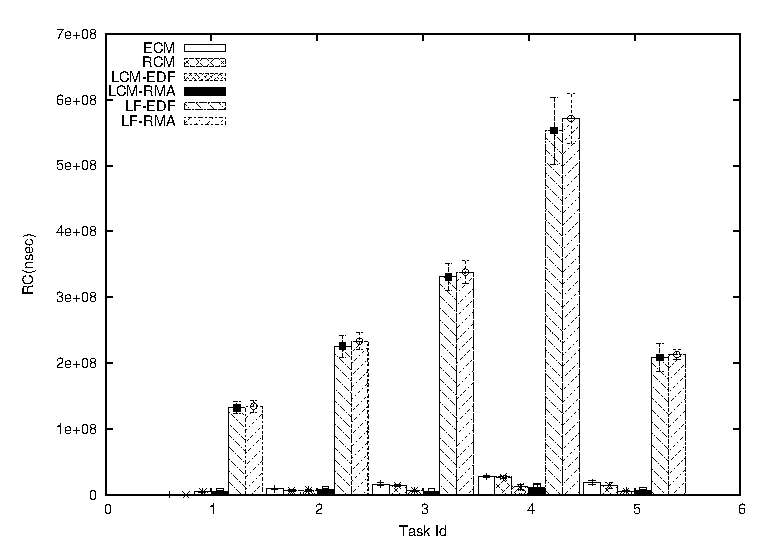
\includegraphics[scale=0.6]
{figures/Abr_dur_5t_nl_g_30_0.2_0.2_0.2_1.eps}
\label{fig-RC-set1}
}
\subfigure[Task set 2]{
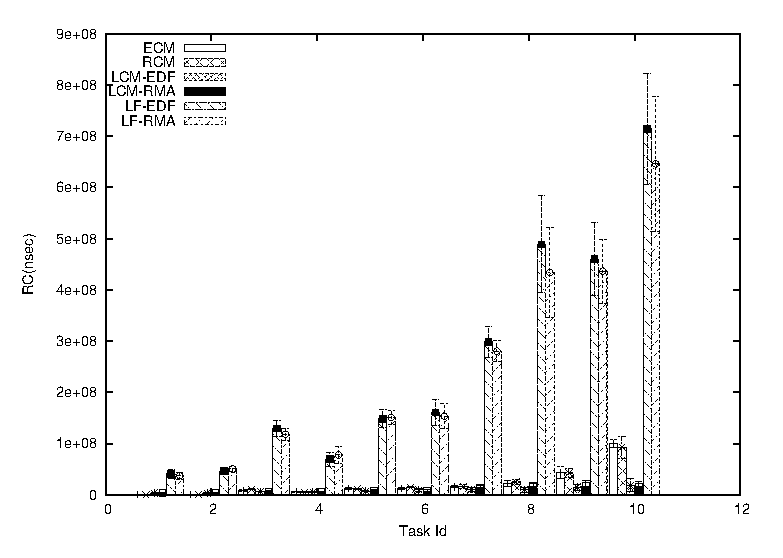
\includegraphics[scale=0.6]{figures/Abr_dur_10t_nl_g_30_0.2_0.2_0.2_1.eps}
\label{fig-RC-set2}
}
\subfigure[Task set 3]{
\includegraphics[scale=0.6]{figures/Abr_dur_12t_nl_g_30_0.2_0.2_0.2_1.eps}
\label{fig-RC-set3}
}
\caption{Task retry costs under LCM and competitor synchronization methods}
\label{fig:RC_results}
\end{figure}

Figure \ref{fig:res_results-1} shows the response time of each task of the task sets in Table \ref{tab:Task-set-1} with a confidence level of 0.95. (Again, each task's atomic section length is equal to half of the task length.) 
We observe that G-EDF/LCM and G-RMA/LCM achieve shorter 
response time than the retry-loop lock-free
algorithm, and shorter 
or comparable response time than ECM and RCM.

\begin{figure}[htbp]
\subfigure[Task set 1]{
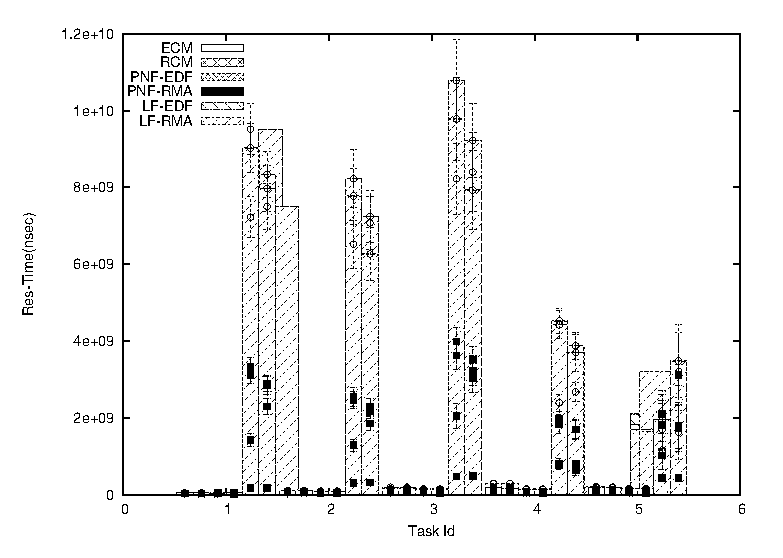
\includegraphics[scale=0.6]{figures/Res_Time_5t_nl_g_30_0.2_0.2_0.2_1.eps}
\label{fig-res-set1-1}
}
\subfigure[Task set 2]{
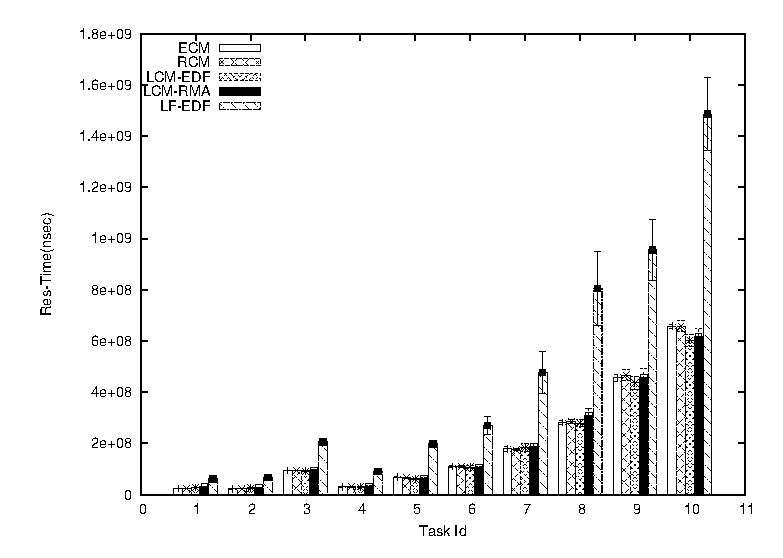
\includegraphics[scale=0.6]{figures/Res_Time_10t_nl_g_30_0.2_0.2_0.2_1.eps}
\label{fig-res-set2-1}
}
\subfigure[Task set 3 ]{
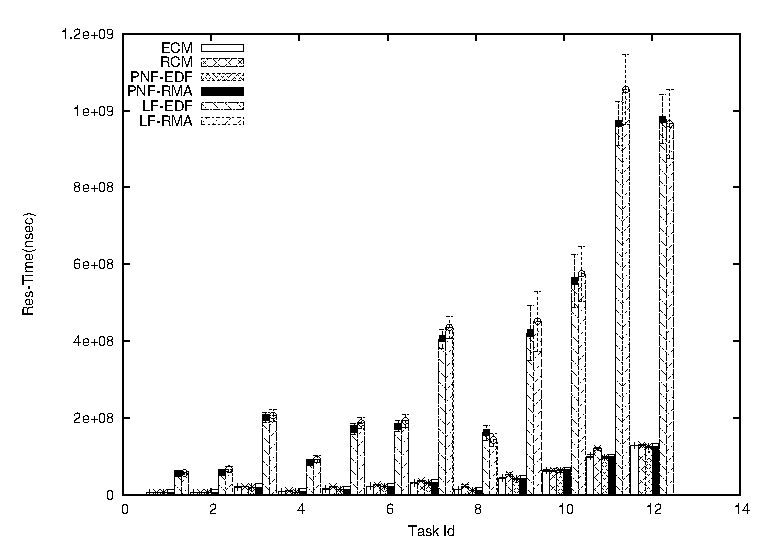
\includegraphics[scale=0.6]{figures/Res_Time_12t_nl_g_30_0.2_0.2_0.2_1.eps}
\label{fig-res-set3-1}
}
\caption{Task response times under LCM and competitor synchronization methods}
\label{fig:res_results-1}
\end{figure}

We repeated the experiments by varying the number and length of atomic sections. Due to space limitation, only subset of results are shown in Figures~\ref{fig:RC_results 5 2 2} to~\ref{fig:res_results 8 5 2}. 
%NEWNEW-start
A complete set of results are shown in Appendix B in~\cite{stmconcurrencycontrol_techreport}. Each figure has three parameters $x,y,z$ in the lable. $x$ specifies the relative total length of all atomic sections to the length of the task. $y$ specifies the maximum relative length of any atomic section to the length of the task. $z$ specifies the minimum relative length of any atomic section to the length of the task. These figures show a consistent trend with previous results.
%NEWNEW-end

\begin{figure}[htbp]
\centering
\subfigure[Task set 1]{
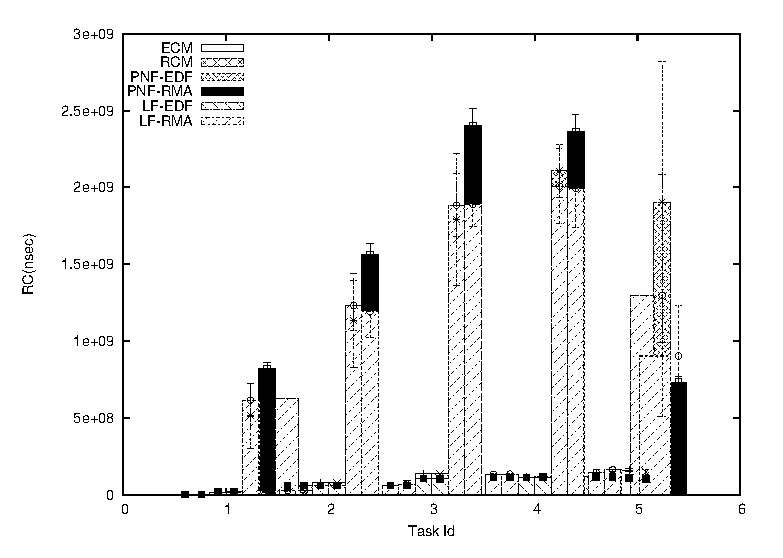
\includegraphics[scale=0.6]
{figures/Abr_dur_5t_nl_g_30_0.5_0.2_0.2_1.eps}
\label{fig-RC-set1}
}
\subfigure[Task set 2]{
\includegraphics[scale=0.6]{figures/Abr_dur_10t_nl_g_30_0.5_0.2_0.2_1.eps}
\label{fig-RC-set2}
}
\subfigure[Task set 3]{
\includegraphics[scale=0.6]{figures/Abr_dur_12t_nl_g_30_0.5_0.2_0.2_1.eps}
\label{fig-RC-set3}
}
\caption{Task retry costs under LCM and competitor synchronization methods (0.5,0.2,0.2)}
\label{fig:RC_results 5 2 2}
\end{figure}

\begin{figure}[htbp]
\subfigure[Task set 1]{
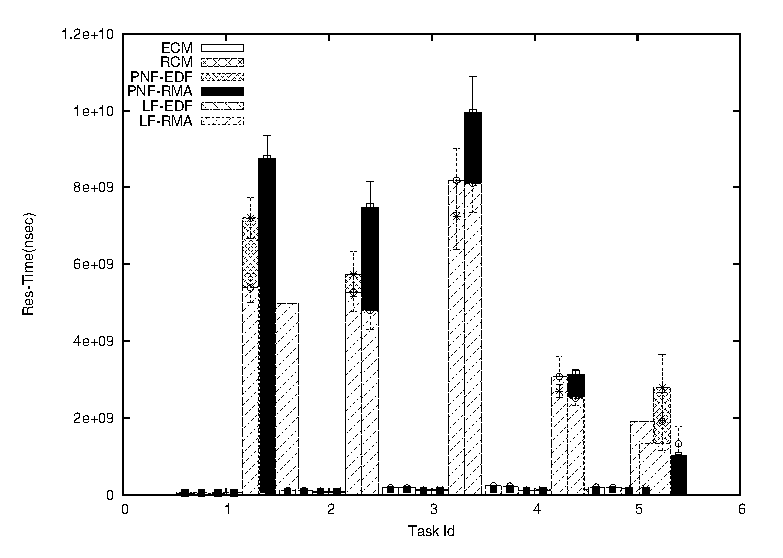
\includegraphics[scale=0.6]{figures/Res_Time_5t_nl_g_30_0.5_0.2_0.2_1.eps}
\label{fig-res-set1-1}
}
\subfigure[Task set 2]{
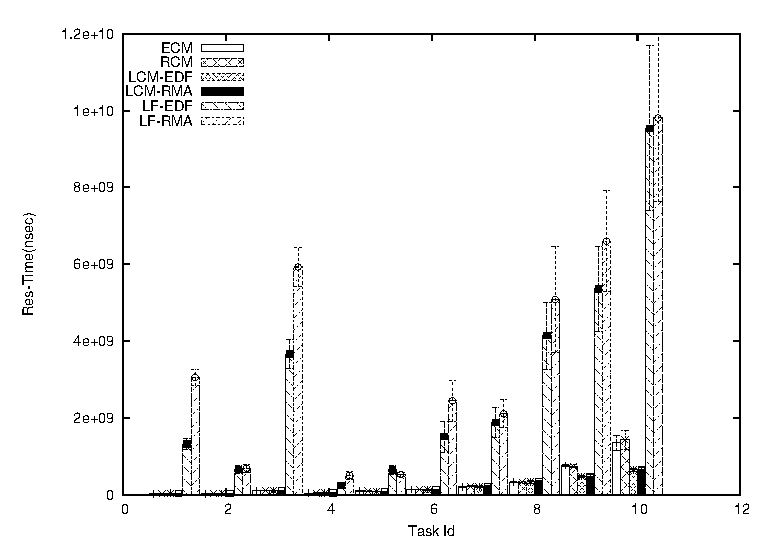
\includegraphics[scale=0.6]{figures/Res_Time_10t_nl_g_30_0.5_0.2_0.2_1.eps}
\label{fig-res-set2-1}
}
\subfigure[Task set 3 ]{
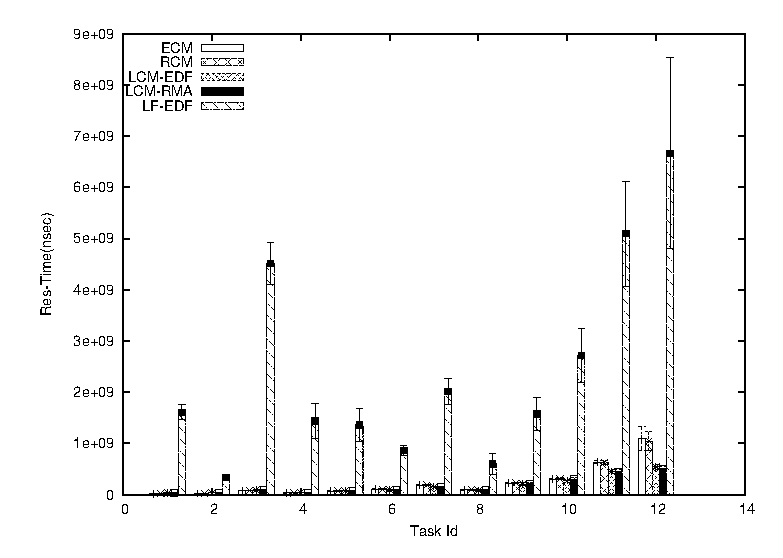
\includegraphics[scale=0.6]{figures/Res_Time_12t_nl_g_30_0.5_0.2_0.2_1.eps}
\label{fig-res-set3-1}
}
\caption{Task response times under LCM and competitor synchronization methods (0.5,0.2,0.2)}
\label{fig:res_results 5 2 2}
\end{figure}

\begin{figure}[htbp]
\centering
\subfigure[Task set 1]{
\includegraphics[scale=0.6]
{figures/Abr_dur_5t_nl_g_30_0.8_0.5_0.2_1.eps}
\label{fig-RC-set1}
}
\subfigure[Task set 2]{
\includegraphics[scale=0.6]{figures/Abr_dur_10t_nl_g_30_0.8_0.5_0.2_1.eps}
\label{fig-RC-set2}
}
\subfigure[Task set 3]{
\includegraphics[scale=0.6]{figures/Abr_dur_12t_nl_g_30_0.8_0.5_0.2_1.eps}
\label{fig-RC-set3}
}
\caption{Task retry costs under LCM and competitor synchronization methods (0.8,0.5,0.2)}
\label{fig:RC_results 8 5 2}
\end{figure}

\begin{figure}[htbp]
\subfigure[Task set 1]{
\includegraphics[scale=0.6]{figures/Res_Time_5t_nl_g_30_0.8_0.5_0.2_1.eps}
\label{fig-res-set1-1}
}
\subfigure[Task set 2]{
\includegraphics[scale=0.6]{figures/Res_Time_10t_nl_g_30_0.8_0.5_0.2_1.eps}
\label{fig-res-set2-1}
}
\subfigure[Task set 3 ]{
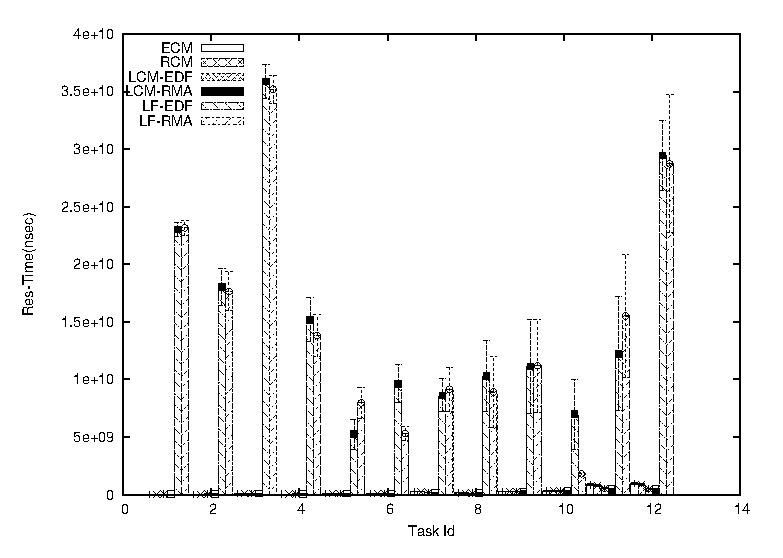
\includegraphics[scale=0.6]{figures/Res_Time_12t_nl_g_30_0.8_0.5_0.2_1.eps}
\label{fig-res-set3-1}
}
\caption{Task response times under LCM and competitor synchronization methods (0.8,0.5,0.2)}
\label{fig:res_results 8 5 2}
\end{figure}



\section{Conclusions}
\label{sec:conclusions_lcm}

In ECM and RCM, a task incurs at most $2s_{max}$ retry cost for each of its atomic section due to conflict
with another task's atomic section. With LCM, this retry cost is reduced to $(1+\alpha_{max})s_{max}$ for each aborted atomic section. In ECM and RCM, tasks do not retry due to lower priority tasks, whereas in LCM, they do so. In G-EDF/LCM, retry due to a lower priority job is encountered only from a task $\tau_{j}$'s last job instance 
during $\tau_{i}$'s period. This is not the case with G-RMA/LCM, because,  each higher priority task can be aborted and retried by any job instance of lower priority tasks. Schedulability of G-EDF/LCM and G-RMA/LCM is better or equal to ECM and RCM, respectively, by proper choices for $\alpha_{min}$ and $\alpha_{max}$. Schedulability of G-EDF/LCM is better than retry-loop lock-free synchronization for G-EDF if the upper bound on $s_{max}/r_{max}$ is between 0.5 and 2, which is higher than that achieved by ECM. 
%sh-new-start
G-RMA/LCM acheives higher schedulability than retry-loop lock-free if $s_{max}/r_{max}$ is not less than 0.5. For high values of $\alpha$ in G-RMA/LCM, $s_{max}/r_{max}$ can extend to large values.
%sh-new-end

\bibliography{/e/lectures/real-time/PhD-work/STM/writing/global_bibliography/global_bibliography.bib}
\end{document}
